% This is a general template file for the LaTeX package SVJour3
% for Springer journals. Original by Springer Heidelberg, 2010/09/16
%
% Use it as the basis for your article. Delete % signs as needed.
%
% This template includes a few options for different layouts and
% content for various journals. Please consult a previous issue of
% your journal as needed.
%
\RequirePackage{fix-cm}
%
%\documentclass{svjour3}                     % onecolumn (standard format)
%\documentclass[smallcondensed]{svjour3}     % onecolumn (ditto)
%\documentclass[smallextended]{svjour3}       % onecolumn (second format)
\documentclass[twocolumn]{svjour3}          % twocolumn
%
\smartqed  % flush right qed marks, e.g. at end of proof
%
\usepackage{graphicx}
\usepackage{amsmath}
\usepackage{amssymb}
%
% insert here the call for the packages your document requires
%\usepackage{mathptmx}      % use Times fonts if available on your TeX system
%\usepackage{latexsym}
% etc.
%
% Jag's 
\usepackage{tabu}
\usepackage{cancel}
\usepackage{algorithm}
\usepackage{algorithmicx}
\usepackage{algpseudocode}
%\usepackage[caption=false]{subfig}
\usepackage{subcaption}
\usepackage{booktabs, mathtools}
\usepackage[dvipsnames]{xcolor}

\captionsetup{compatibility=false}

\algdef{SE}[DOWHILE]{Do}{doWhile}{\algorithmicdo}[1]{\algorithmicwhile\ #1}%

\DeclareMathOperator{\Order}{{\mathcal O}}

% please place your own definitions here and don't use \def but
% \newcommand{}{}
\providecommand{\HickernellFJ}{Hickernell}
\newcommand{\bm}[1]{\boldsymbol{#1}}
\newcommand{\mSigma}{\Sigma}
\newcommand{\mB}{\mathsf{B}}
\newcommand{\smallocite}[1]{{\small\ocite{#1}}}
% \newcommand{\bm}[1]{\boldsymbol{#1}}
\newcommand{\dif}[1]{\text{d}{#1}}
\newcommand{\D}[1]{\text{d}{#1}}
\newcommand{\trace}[1]{\textup{trace}{#1}}

\newcommand{\naturals}{\mathbb{N}}
\newcommand{\reals}{\mathbb{R}}
\newcommand{\integers}{\mathbb{Z}}
\newcommand{\posIntegers}{\mathbb{Z}_{> 0}}
\newcommand{\complex}{\mathbb{C}}
\newcommand{\hilbert}{\mathbb{H}}
\newcommand{\Ex}{\mathbb{E}}

\newcommand{\cf}{\mathcal{F}}
\newcommand{\cx}{\mathcal{X}}
\newcommand{\tcx}{\widetilde{\cx}}

\newcommand{\valpha}{{\bm{\alpha}}}
\newcommand{\vbeta}{{\bm{\beta}}}
\newcommand{\vlambda}{{\bm{\lambda}}}
\newcommand{\vphi}{{\bm{\phi}}}
\newcommand{\vpsi}{{\bm{\psi}}}
\newcommand{\vtheta}{{\bm{\theta}}}
\newcommand{\vzeta}{{\bm{\zeta}}}
\newcommand{\vthetaMLE}{\bm{\theta}_{\text{MLE}}}
\newcommand{\hvtheta}{\hat{\vtheta}}
\newcommand{\va}{\bm{a}}
\newcommand{\vA}{\bm{A}}
\newcommand{\vb}{\bm{b}}
\newcommand{\vc}{\bm{c}}
\newcommand{\vC}{\bm{C}}
\newcommand{\tvc}{\tilde{\bm{c}}}
\newcommand{\vg}{\bm{g}}
\newcommand{\vh}{\bm{h}}
\newcommand{\vf}{\bm{f}}
\newcommand{\vk}{\bm{k}}
\newcommand{\vm}{\bm{m}}
\newcommand{\vs}{\bm{s}}
\newcommand{\vt}{\bm{t}}
\newcommand{\vv}{\bm{v}}
\newcommand{\vV}{\bm{V}}
\newcommand{\vw}{\bm{w}}
\newcommand{\vW}{\bm{W}}
\newcommand{\vx}{\bm{x}}
\newcommand{\dx}{\dif{{x}}}
\newcommand{\dt}{\dif{{t}}}
\newcommand{\dvx}{\dif{\bm{x}}}
\newcommand{\dvs}{\dif{\bm{s}}}
\newcommand{\dvt}{\dif{\bm{t}}}
\newcommand{\vrho}{\bm{\rho}}
\newcommand{\hy}{\hat{y}}
\newcommand{\vy}{\bm{y}}
\newcommand{\vY}{\bm{Y}}
\newcommand{\hvy}{\hat{\vy}}
\newcommand{\vz}{\bm{z}}
\newcommand{\vZ}{\bm{Z}}
\newcommand{\dvz}{\dif{\bm{z}}}
\newcommand{\tf}{\tilde{f}}

\newcommand{\tvv}{\tilde{\vv}}
\newcommand{\tvz}{\tilde{\vz}}

\newcommand{\vCvtheta}{{C_\vtheta}}
\newcommand{\hc}{\widehat{c}}

\newcommand{\hatvy}{\hat{\bm{y}}}
\newcommand{\haty}{\hat{y}}
\newcommand{\tvy}{\tilde{\bm{y}}}
\newcommand{\ty}{\tilde{y}}
\newcommand{\vzero}{\bm{0}}
\newcommand{\vone}{\bm{1}}
\newcommand{\tvone}{\tilde{\bm{1}}}
\newcommand{\mA}{\mathsf{A}}
\newcommand{\mC}{\mathsf{C}}
\newcommand{\mCtheta}{{\mathsf{C}_{\vtheta}}}
%\newcommand{\mCthetaInv}{{\mathsf{C}^{-1}_{\vtheta}}}
%\newcommand{\mCthetaMLE}{{\mathsf{C}_{\vthetaMLE}}}
%\newcommand{\mCthetaInvMLE}{{\mathsf{C}^{-1}_{\vthetaMLE}}}
\newcommand{\mCInv}{{\mathsf{C}^{-1}}}
\newcommand{\cov}{{\textup{cov}}}
\newcommand{\var}{{\textup{var}}}


\newcommand{\tmC}{\widetilde{\mathsf{C}}}
\newcommand{\tlambda}{\tilde{\lambda}}

\newcommand{\mL}{\mathsf{L}}

\newcommand{\mLambda}{\mathsf{\Lambda}}
\newcommand{\mLambdaInv}{\mathsf{\Lambda}^{-1}}

\newcommand{\mV}{\mathsf{V}}
\newcommand{\mW}{\mathsf{W}}

\newcommand{\calN}{\mathcal{N}}

\newcommand{\tvrho}{\widetilde{\vrho}}
\newcommand{\heta}{\hat{\eta}}
\newcommand{\hmu}{\widehat{\mu}}
\newcommand{\hsigma}{\widehat{\sigma}}
\newcommand{\hnu}{\hat{\nu}}
\newcommand{\rhoCond}{\mathring{\vrho}}

\newcommand{\MLE}{\text{MLE}}
%\newcommand{\errtol}{\text{tol}}
\newcommand{\errtol}{\varepsilon}
\newcommand{\errn}{\text{err}_{n}}
\newcommand{\diag}{\text{diag}}
\newcommand{\err}{\textup{err}}

\def\abs#1{\ensuremath{\left \lvert #1 \right \rvert}}
\newcommand{\norm}[2][{}]{\ensuremath{\left \lVert #2 \right \rVert}_{#1}}
\newcommand{\ip}[3][{}]{\ensuremath{\left \langle #2, #3 \right \rangle_{#1}}}

\newenvironment{nalign}{
    \begin{equation}
    \begin{aligned}
}{
    \end{aligned}
    \end{equation}
    \ignorespacesafterend
}

\providecommand{\argmin}{\operatorname*{argmin}}
\providecommand{\argmax}{\operatorname*{argmax}}
\newcommand\figref{Figure~\ref}

\graphicspath{{./figures/}{D:/Mega/MyWriteupBackup/Sep_2ndweek_1/}}
%\graphicspath{{./figures/}}

%
% Insert the name of "your journal" with
% \journalname{myjournal}
%

\newcommand{\FJHNote}[1]{{\textcolor{blue}{FJH: #1}}}
\newcommand{\JRNote}[1]{{\textcolor{green}{JR: #1}}}


\allowdisplaybreaks[4]
\begin{document}
\setlength\abovedisplayskip{1pt}
\setlength{\belowdisplayskip}{1pt}

\title{Fast Automatic Bayesian Cubature Using Lattice Sampling
%\thanks{}
}
% Grants or other notes about the article that should go on the front
% page should be placed within the \thanks{} command in the title
% (and the %-sign in front of \thanks{} should be deleted)
%
% General acknowledgments should be placed at the end of the article.

%\subtitle{Do you have a subtitle?\\ If so, write it here}

%\titlerunning{Short form of title}        % if too long for running head

\author{R. Jagadeeswaran         \and
        Fred. J. Hickernell %etc.
}

%\authorrunning{Short form of author list} % if too long for running head

\institute{F. Author \at
              first address \\
              Tel.: +123-45-678910\\
              Fax: +123-45-678910\\
              \email{fauthor@example.com}           %  \\
%             \emph{Present address:} of F. Author  %  if needed
           \and
           S. Author \at
              second address
}

\date{Received: date / Accepted: date}
% The correct dates will be entered by the editor

\maketitle

\begin{abstract}
Automatic cubatures provide approximations to multidimensional integrals that satisfy user-specified error tolerances.  For multidimensional problems, the sampling density is fixed, but the
sample size, $n$, is determined automatically. Bayesian cubature postulates that the integrand is an instance of a stochastic process.
Prior information about mean and covariance of this process is used to form data-driven error bounds.  However, the process of inferring the mean and covariance governing the stochastic process from $n$ integrand values involves computing matrix inverses and determinants,
which are in general time-consuming $O(n^3)$ operations.
Our work employs low discrepancy data sites and matching kernels that lower the  computational cost to $O(n \log n)$.  The confidence interval for the Bayesian posterior error is used to choose $n$ automatically to satisfy the user-defined error tolerance.  This approach is demonstrated using rank-1 lattice sequences and shift-invariant kernels.

%Include keywords, PACS, and mathematical subject classification numbers as needed.

\keywords{Bayesian cubature \and Probabilistic numeric methods \and GAIL}
% \PACS{PACS code1 \and PACS code2 \and more}
% \subclass{MSC code1 \and MSC code2 \and more}
\end{abstract}

\section{Introduction}
\label{intro}
Cubature is the problem of inferring a numerical value for the integral 
$\mu = \int_{\reals^d} g(\vx) \, \dif \vx$, of a multi-dimensional function $g$ where $\mu$ has no closed form analytic expression. Typically, $g$ is only accessible in the form of a black-box function routine. 
Cubature is a key component of many problems in scientific computing, finance, statistical modeling, and machine learning.  
%One could use Numerical algorithms to estimate quantities that can not be directly computed, using the results of %more readily available computations.


%Multivariate integrals arise in applications such as evaluating financial risk, computing multivariate probabilities, statistical physics, and uncertainty quantification.


The integral $\mu$ may often be expressed in the form
\begin{equation}
\label{eqn:defn_mu}
\mu:= \mu(f) := \Ex[f(\boldsymbol{X})] = \int_{[0,1]^d} f(\vx)\, \dif\vx, 
\end{equation}
where $f:[0,1]^d \to \reals$ is the integrand, and $\boldsymbol{X} \sim \mathcal{U}[0,1]^d$.  The problem of transforming the original integral into the above form is not addressed here.  The cubature algorithm may take the form
\begin{equation}
\label{eqn:defn_hmu}  % remove this
\hmu: = \hmu(f) := w_0 + \sum_{i=1}^{n} f(\vx_i) w_i,
\end{equation}
where the weights, $w_0$, and  $\vw = (w_i)_{i=1}^n \in \reals^n$, and the nodes, $\{x_i\}_{i=1}^n \subset [0,1]^d$, are chosen to make the error, $\abs{\mu - \hmu}$, small.  In this article the nodes is assumed to be deterministic.

Our concern is constructing a reliable stopping criterion that determines the number of integrand values required, $n$, to ensure that the error is no greater than a user-defined error tolerance, i.e., 
\begin{equation}
\label{eqn:err_crit} 
\abs{\mu - \hmu} \leq \errtol 
\end{equation}
Rather than relying on strong assumptions about the integrand, such as its variance or total variation, we construct a stopping criterion that is data-driven, and based on a credible interval arising from a Bayesian approach to the problem.  We build upon the ideas of Diaconis\cite{DiaconisBayesian}, O'Hagan\cite{HagenBayes}, Ritter\cite{RiterAverage}, Rasmussen and Ghahramani\cite{RasmussenBayesian}, Briol et al.\cite{BriEtal18a}, and others.  Thus, our algorithm is an example of \emph{probabilistic numerics}.

Our primary contribution here is to demonstrate how the choice of a family of kernels that match the low discrepancy sampling nodes facilitates fast computation of the data-driven stopping criterion.  If $n$ function values, at a cost of $\$(f)$ each, are obtained for cubature purposes, then $\Order(n \log(n))$ additional operations are required to check whether the error tolerance is satisfied.  The total cost of our algorithm is then $\Order(\$(f)n + n \log(n))$.  This is significantly fewer operations than the $\Order(n^3)$ typically required for Bayesian cubature.

Hickernell \cite{Hic17a} compares and contrasts different approaches to cubature error analysis depending on whether the rule is deterministic or random and whether the integrand is assumed to be deterministic or random.  Error analyis that assumes a deterministic integrand lying in a Banach space, leads to an error bound that is typically impractical for deciding how large $n$ must be to satisfy \eqref{eqn:err_crit}.  The deterministic error bound includes a (semi-)norm of the integrand, which is often more complex to compute than the original integral.

Hickernell and Jim\'enez-Rugama\cite{HicJim16a,JimHic16a} have developed stopping criteria for cubature rules based on low discrepancy nodes by tracking the discrete Fourier coefficients of the integrand.  The algorithm proposed here also depends on the discrete Fourier coefficients of the integrand, but in a different way.

Section \ref{sec:BC} explains the Bayesian approach to estimate the posterior cubature error and defines our automatic Bayesian cubature . Although much of this material is not new, it is included for completeness.  We end Section \ref{sec:BC}  by demonstrating why Bayesian cubature is typically quite computationally expensive.
Section \ref{sec:fast_BC}  introduces the concept of covariance kernels that match well the nodes and expedites the computations required by our automatic Bayesian cubature. 
Section \ref{sec:shift_invariant_kernel} implements this idea for shift invariant kernels and rank-1 lattice nodes.
Section 5 covers further enhancements to the algorithm to avoid cancellation error and make it faster. Finally, numerical examples are shown using the faster algorithm developed.



\section{Bayesian cubature} \label{sec:BC}
\label{sec:1}
%Text with citations \cite{RefB} and \cite{RefJ}.

\subsection{Bayesian posterior error}
\label{sec:BayesPostErr}

Suppose that the integrand, $f$, is drawn from a Gaussian process, i.e., $f \sim \mathcal{GP}(m,s^2 C_\vtheta)$.  Specifically, $f$ has real-valued mean $m$ and covariance function $s^2C_\vtheta$, where $s$ is a non-negative scale factor $s$ $C_\vtheta: [0,1]^d \times [0,1]^d \to \mathbb{R} $ is a symmetric, positive-definite function and parameterized by $\vtheta$:
\begin{multline} \label{FJH:eq:CondPosDef}
\mC^T = \mC,  \qquad \va^T \mC \va > 0 \quad  \forall \va \ne \vzero, 
\\ \text{where } \mC = \left(  C_\vtheta(\vx_i,\vx_j)  \right)_{i,j=1}^n,\\
\forall n\in \mathbb{N}, \; \vt, \vx, \vx_1, \ldots, \vx_n \in [0,1]^d.
\end{multline}
The covariance function, $C$, and the Gram matrix, $\mC$ depend implicitly on $\vtheta$, but sometimes this is omitted in the notation for simplicity's sake.

For a Gaussian process, all vectors of linear functionals of $f$ have a multivariate Gaussian distribution. Defining  $\vf  := \left( f(\vx_i)\right)_{i=1}^n$ as the multivariate normal vector of function values, it follows that 
\begin{subequations}
\begin{align}
\label{eqn:fGaussDist}
\vf  & \sim \calN(m \vone, s^2 \mC), \\
\mu & \sim \calN(m, s^2 c_0), 
\\
\text{where }
c_0 &= \int_{[0,1]^{2d}} C_\vtheta(\vx,\vt) \, \dif{\vx} \, \dif{\vt}, \\
\cov(\vf, \mu) &= \left(  \int_{[0,1]^d} C(\vt,\vx_i) \, \D \vt \right)_{i=1}^n  =: \vc.
\end{align}
\end{subequations}
Therefore,  it follows from \cite{RasWil06a} Appendix A.2 Gaussian Identities that the \emph{conditional} distribution of the integral given observed function values, $\vf = \vy$ is also Gaussian:
\begin{multline} \label{eqn:condInteg}
\mu | (\vf = \vy) \sim \calN \bigl(m (1 - \vc^T \mC^{-1} \vone)  + \vc^T \mC^{-1} \vy, 
\\
s^2(c_0  -\vc ^T \mC^{-1} \vc) \bigr).
\end{multline}

The natural choice for  the cubature is the posterior mean of the integral, namely, 
\begin{equation}
\label{eqn:BayesCub}
\widehat{\mu}  \vert ( \vf = \vy)
= m(1 - \vone^T  \mC^{-1}\vc )
+ \vc^T \mC^{-1} \vy.
\end{equation}
Under this definition, the cubature error has zero mean and a variance depending on the choice of nodes:
\begin{equation*}
%\label{eqn_error_cond_prob}
(\mu-\hmu) | (\vf = \vy)
 \sim  \calN 
\left(
0, \;
s^2 (c_0 - \vc^T\mC^{-1}\vc) 
\right).
\end{equation*}
A credible interval for the integral is given given by 
\begin{equation}
\label{eqn_prob_confidence_interval}
\mathbb{P}_f \left[
|\mu-\hmu| \leq  2.58 s \sqrt{c_0 - \vc^T\mC^{-1}\vc } 
\right] = 99\%.
\end{equation}
Natually, the $2.58$ and $99\%$ can be replaced by other quantiles and credible levels.


\subsection{Parameter estimation}
The credible interval in \eqref{eqn_prob_confidence_interval} suggests how our automatic Bayesian cubature proceeds.  Function data is accumulated until we can be confident that the error is no greater than the error tolerance.  However, the credible interval still depends on the parameters $m, s$, and $\vtheta$.  These should not be assumed a priori but be inferred from the data.  This section describes three approaches.

\subsubsection{Empirical Bayes}  \label{sec:MLE}
One approach to estimate the parameters is via maximum likelihood estimation (MLE).  The log-likelihood function of the parameters given the function data $\vy$ is:
\begin{multline}
l(s,m,\vtheta | \vy)
= -\frac{1}{2} s^{-2} (\vy-m\vone)^T\mCInv(\vy-m\vone) 
\\
 - \frac{1}{2} \log(\det\, \mC) - \frac{n}{2} \log(s^2) + \text{constants.}
\end{multline}
Maximizing the log-likelihood first with respect to $m$, then with respect to $s$, and finally with respect to $\vtheta$ yields
\begin{align}
\label{eqn_m_MLE}
m_\MLE &= \frac{\vone^T \mCInv \vy }{ \vone^T \mCInv \vone} \\
\nonumber
s^2_{\MLE}  
&= \frac{1}{n} (\vy-m_{\MLE}\vone)^T\mCInv(\vy-m_{\MLE}\vone) 
\\
\label{eqn_s2_MLE}
&= 
\frac{1}{n}
\vy^T 
\left[ 
\mCInv - 
\frac{ \mCInv \vone \vone^T \mCInv }{\vone^T\mCInv \vone}
\right] \vy, \\
\nonumber
\vtheta_\MLE
&= \argmin_{\vtheta} \biggl \{
\log\left(\vy^T 
\left[ \mCInv - 
\frac{ \mCInv \vone \vone^T \mCInv }{\vone^T\mCInv \vone}
\right] \vy 
\right)  \\
\label{eqn:thetaMLE}
 & \qquad +  \frac{1}{n} \log(\det(\mC))
\biggr \}.
\end{align}
The MLE estimate of $\vtheta$ balances minimizing the covariance scale factor, $s^2_{\MLE}$, against minimizing  $\det(\mC)$. 

Under these estimates of the parameters, the cubature \eqref{eqn:BayesCub} and the credible interval \eqref{eqn_prob_confidence_interval} simplify to 
\begin{align} \label{eqn:cubMLE}
\hmu_\MLE  &= 
\left(
\frac{ (1 - \vone^T  \mCInv\vc )  \vone }{ \vone^T \mCInv \vone}   +  \vc 
\right)^T  \mCInv \vy, \\
 \label{eqn:errMLE}
\err_\MLE^2 & : = \frac{2.58^2}{n}
 \vy^T \left[ \mCInv - 
\frac{ \mCInv \vone \vone^T \mCInv }{\vone^T\mCInv \vone}
\right] \vy \\
&\qquad \qquad \times 
(c_0 - \vc^T\mC^{-1}\vc ),
\end{align}
\begin{equation}
\label{eqn_prob_CI_MLE}
\mathbb{P}_f \left[
|\mu-\hmu_\MLE| \leq \err_\MLE \right]  = 99\%.
\end{equation}
Here $c_0$, $\vc$, and $\mC$ are assumed implicitly to be based on $\vtheta = \vtheta_\MLE$.   

\subsubsection{Full Bayes}

Rather than use maximum likelihood to determine $m$ and $s$ one treat them as hyper-parameters and may a non-informative, conjugate prior, namely $\vrho_{m,s^2}(\xi, \lambda) \propto 1/\lambda$. Then the posterior density for the integral given the data using Bayes theorem is
\begin{align*}
\MoveEqLeft[1]{\rho_{\mu}(z | \vf = \vy)} \\
& \propto \int_{0}^\infty \int_{-\infty}^\infty \rho_{\mu}(z | \vf = \vy, m = \xi, s^2 = \lambda) \\
& \qquad \qquad \times  \rho_{\vf}(\vy | \xi, \lambda ) \rho_{m, s^2}(\xi, \lambda) \, \D \xi \D \lambda \\
& \propto \displaystyle \int_{0}^\infty  \frac{1}{\lambda^{(n+3)/2}} \\
& \times \int_{-\infty}^\infty  \exp \biggl( -\frac{1}{2\lambda}\biggl\{
\frac{
[z - \xi (1 - \vc^T \mC^{-1} \vone)  -  \vc^T \mC^{-1} \vy]^2}
{c_0  -\vc ^T \mC^{-1} \vc}  \\
& \qquad \qquad  + (\vy - \xi \vone)^T \mC^{-1}(\vy - \xi \vone) \biggr \} \biggr) \, \D \xi \D \lambda \\
&\qquad \qquad
\text{by \eqref{eqn:fGaussDist}, \eqref{eqn:condInteg}} \; \text{and} \; \rho_{m,s^2}(\xi,\lambda) \propto 1/\lambda \\
& \propto \displaystyle \int_{0}^\infty  \frac{1}{\lambda^{(n+3)/2}} \cdots \\ & \qquad \cdots \int_{-\infty}^\infty  \exp\left( -\frac{\alpha \xi^2 -2 \beta \xi + \gamma}{2\lambda(c_0  -\vc ^T \mC^{-1} \vc)} \right) \, \D \xi \D \lambda, \\
\intertext{where}
\alpha & = (1 - \vc^T \mC^{-1} \vone)^2 + \vone^T \mC^{-1} \vone (c_0  -\vc ^T \mC^{-1} \vc),\\
\beta & =(1 - \vc^T \mC^{-1} \vone)(z - \vc^T \mC^{-1} \vy ) \\
& \qquad \qquad  + \vone^T \mC^{-1} \vy (c_0  -\vc ^T \mC^{-1} \vc),\\
\gamma &  = (z - \vc^T \mC^{-1} \vy )^2  + \vy^T \mC^{-1} \vy (c_0  -\vc ^T \mC^{-1} \vc).
\end{align*}
In the derivation above and below, factors that are independent of $\xi$, $\lambda$, or $z$ can be discarded since we only need to preserve the proportion, however, factors that depend on $\xi$, $\lambda$, or $z$ must be kept.  
%Completing the square allows us to compute the integral with respect to $\xi$:
Completing the square $
\alpha \xi^2 -2 \beta \xi + \gamma 
= \alpha (\xi -\beta/\alpha)^2  - (\beta^2/\alpha) + \gamma,
$
allows us to evaluate the integrals with respect to $\xi$ and $\lambda$:
\begin{align*}
\MoveEqLeft{\rho_{\mu}(z | \vf = \vy)} \\
& \propto \displaystyle \int_{0}^\infty  \frac{1}{\lambda^{(n+3)/2}}  \exp\left( -\frac{  \gamma - \beta^2/\alpha}{2\lambda(c_0  -\vc ^T \mC^{-1} \vc)} \right)  \cdots \\
& \qquad \qquad \cdots \int_{-\infty}^\infty  \exp\left( -\frac{\alpha (\xi -\beta/\alpha)^2}{2\lambda(c_0  -\vc ^T \mC^{-1} \vc)} \right) \, \D \xi \D \lambda \\
& \propto \displaystyle \int_{0}^\infty  \frac{1}{\lambda^{(n+2)/2}}  \exp\left( -\frac{  \gamma - \beta^2/\alpha}{2\lambda(c_0  -\vc ^T \mC^{-1} \vc)} \right) \D \lambda \\
& \propto \left(\gamma - \frac{\beta^2}{\alpha}\right)^{-n/2} \propto \left(\alpha \gamma - \beta^2\right)^{n/2}.
\end{align*}
Finally, we simplify the key term via straightforward calculations to the following:
\begin{equation*}
\alpha \gamma - \beta^2 \propto 1 +  \frac{(z - \hmu_{\textup{MLE}})^2}{(n-1)\widehat{\sigma}_{\textup{full}}^2}, \\
\end{equation*}
where 
\begin{multline}
\label{FJH:eq:signmaFull}
\hsigma^2_{\textup{full}} 
:= \frac{1}{n-1}
\vy^T\left[ \mC^{-1} 
- \frac{ \mC^{-1} \vone\vone^T \mC^{-1}}{\vone^T \mC^{-1} \vone}  \right]\vy
\\ 
\times  \left[\frac{(1 - \vc^T \mC^{-1} \vone)^2}{\vone^T \mC^{-1} \vone} + (c_0  -\vc ^T \mC^{-1} \vc) \right].
\end{multline}

This means that $\mu \vert (\vf = \vy )$, properly centered and scaled, has a Student's $t$-distribution with $n-1$ degrees of freedom.   The estimated integral is the same as in the empirical Bayes case, but the confidence interval is wider:
\begin{equation}
\label{eqn_prob_CI_full}
\mathbb{P}_f \left[
|\mu-\hmu_\MLE| \leq \err_{\textup{full}} \right]  = 99\%,
\end{equation}
where
\begin{equation}
\label{FJH:eq:errFull}
\err_{\textup{full}} 
:= t_{n_j-1,0.995} \hsigma_{\textup{full}} > \err_\MLE .
\end{equation}
Here $t_{n-1,0.995}$ denotes the $99.5$ percentile of a standard Student's $t$-distribution with $n-1$ degrees of freedom.

Because the shape parameter, $\vtheta$, enters the definition of the covariance kernel in a non-trivial way, the only way to treat it as a hyperparameter and assign a tractable prior would be for the prior to be discrete.  We believe in practice that choosing such a prior involves more guesswork than using the empirical Bayes estimate of $\vtheta$ in \eqref{eqn:thetaMLE} or the cross-validation approached described next.


\subsubsection{Generalized Cross-validation} \label{sec:GCV}
A third parameter optimization is \emph{leave-one-out cross-validation}.  Let $\widetilde{y}_i = \Ex[f(\vx_i ) | \vf_{-i} = \vy_{-i}]$, where the subscript $-i$ denotes the vector excluding the $i^{\text{th}}$ component.  This is the conditional expectation of $f(\vx_i )$ given all data but the function value at $\vx_i$.  The cross-validation criterion, which is to be minimized, is sum of squares of the difference between these conditional expectations and the observed values:
\begin{equation} \label{FJH:eq:CVA}
\textup{CV} = \sum_{i=1}^n (y_i - \widetilde{y}_i)^2.
\end{equation}

Let $\mA = \mC^{-1}$, let $\vzeta = \mA (\vy - m \vone)$, and partition $\mC$, $\mA$, and $\vzeta$ as
\begin{gather*}
\mC = \begin{pmatrix} c_{ii}  & \vC_{-i,i}^T \\  \vC_{-i,i} & \mC_{-i,-i}\end{pmatrix}, \qquad
\mA = \begin{pmatrix} a_{ii}  & \vA_{-i,i}^T \\  \vA_{-i,i} & \mA_{-i,-i}\end{pmatrix}, \\ \vzeta = \begin{pmatrix} \zeta_i   \\  \vzeta_{-i} \end{pmatrix},
\end{gather*}
where the subscript $i$ denotes the $i^{\text{th}}$ row or column, and the subscript $-i$ denotes all rows or columns except the $i^{\text{th}}$. Following this notation, Lemma \ref{thrm:condDist} implies that 
\begin{align*}
\widetilde{y}_i & = m + \vC^T_{-i,i} \mC_{-i,-i}^{-1} (\vy_{-i} -m \vone)  \\
\zeta_i  & = a_{ii}(y_i - m) + \vA_{-i,i}^T(\vy_{-i} - m \vone) \\
& = a_{ii}[(y_i - m) - \vC^T_{-i,i} \mC_{-i,-i}^{-1} (\vy_{-i} -m \vone)] \\
& = a_{ii}(y_i - \widetilde{y}_i).
\end{align*}
Thus, \eqref{FJH:eq:CVA} may be re-written as 
\begin{equation*} %\label{FJH:eq:CVB}
\textup{CV} = \sum_{i=1}^n \left(\frac{\zeta_i}{a_{ii}} \right)^2, \qquad \vzeta = \mC^{-1}(\vy - m \vone).
\end{equation*}
Wahba \ref{} recommended a generalized cross-validation criterion, which replaces the $i^{\text{th}}$ diagonal element of $\mA$ in the denominator by the average diagonal element of $\mA$:
\begin{align} 
\nonumber
\textup{GCV} &
= \frac{\sum_{i=1}^n\zeta_i^2}{\left(\frac 1n \sum_{i=1}^n a_{ii} \right)^2} \\
\label{FJH:eq:GCV}
& = \frac{(\vy - m\vone)^T \mC^{-2} (\vy - m \vone)}{\left(\frac 1n \trace(\mC^{-1}) \right)^2}.
\end{align}

The loss function $GCV$ depends on $m$ and $\vtheta$, but not on $s$.  Minimizing the GCV  yields
\begin{equation}
m_{\textup{GCV}} = \frac{\vone^T \mC^{-2} \vy}{\vone^T \mC^{-2} \vone},\\ 
\end{equation}
\begin{multline}
\label{vthetaGCV}
\vtheta_{\textup{GCV}} = \argmin_\vtheta \left\{\log \left (  \vy^T \left[\mC^{-2} - \frac{\mC^{-2} \vone \vone^T \mC^{-2}}{\vone^T \mC^{-2} \vone}  \right] \vy \right ) \right . \\
\left . - 2 \log \left ( \trace(\mC^{-1}) \right ) \right\} .
\end{multline}
Plugging this value of $m$ into \eqref{eqn:BayesCub} yields
\begin{equation}
\label{eqn:muCV}
\widehat{\mu}_{\textup{GCV}}
= \left(\frac{(1 - \vone^T  \mC^{-1}\vc) \mC^{-1} \vone}{\vone^T \mC^{-2} \vone} + \vc \right)^T \mC^{-1} \vy.
\end{equation}

An estimate for $s$ may be obtained by noting that by Lemma \ref{thrm:condDist},
\[
\var[f(\vx_i ) | \vf_{-i} = \vy_{-i}] = s^2 a_{ii}^{-1},
\]
Thus, we may estimate $s$ using an argument similar to that used in deriving the GCV and then substituting $m_{\textup{GCV}}$ for $m$:
\begin{align}
\nonumber 
s^2 &= \var[f(\vx_i ) | \vf_{-i} = \vy_{-i}] a_{ii} \\
\nonumber 
& \approx \frac 1n \sum_{i=1}^n (y_i - \widetilde{y}_i)^2a_{ii}
 = \frac 1n \sum_{i=1}^n \frac{\zeta_i^2}{a_{ii}} \\
\nonumber 
 & \approx \frac{ \frac 1n \sum_{i=1}^n \zeta_i^2}{\frac 1n \sum_{i=1}^n a_{ii} } = \frac{(\vy - m\vone)^T \mC^{-2} (\vy - m \vone)}{ \trace(\mC^{-1}) } \\
\nonumber 
 & \approx  s^2_{\textup{GCV}} \\
 \intertext{where}
 \nonumber
 s^2_{\textup{GCV}} & : = \vy^T \left[\mC^{-2} - \frac{\mC^{-2} \vone \vone^T \mC^{-2}}{\vone^T \mC^{-2} \vone}  \right] \vy \\
 &\qquad \qquad  \qquad \qquad  \times \left[ \trace(\mC^{-1}) \right]^{-1} \label{sGCVDef}
\end{align}

The confidence interval based on generalized cross-validation corresponds to \eqref{eqn_prob_confidence_interval} with the GCV estimates for $m$, $s$, and $\vtheta$:
\begin{gather}
\label{GCVerr}
\err_{\textup{GCV}} = 2.58 s_{\textup{GCV}}  \sqrt{c_0 - \vc^T\mC^{-1}\vc} \\
\label{GCVCI}
\mathbb{P}_f \left[
|\mu-\hmu_{\textup{GCV}}| \leq \err_{\textup{GCV}} 
\right] = 99\%.
\end{gather}

Looking back over the results of Sections  \ref{sec:MLE}--\ref{sec:GCV}, it is noted that if  the original covariance function, $C$, is replaced by $b \mC$ for some positive constant $b$, the cubature, $\hmu$, the estimates of $\vtheta$, and the credible interval widths, $\err$, all remain unchanged.  The estimates of $s^2$ are multiplied by $b^{-1}$, as would be expected. 


\subsection{The automatic Bayesian cubature algorithm}
\label{sec:bayes_cubature_algo}
The previous section presents three credible intervals, \eqref{eqn_prob_CI_MLE}, \eqref{eqn_prob_CI_full}, and \eqref{GCVCI}, for the $\mu$, the desired integral.  Each credible interval is based on different assumptions about the hyperparameters $m$, $s$, and $\vtheta$.  We stress that one must estimate these hyperparameters or assume a prior distribution on them because the credible intervals are used as stopping criteria for our cubature rule.  Since a credible intervals makes a statement about a typical function---not an outlier---one must try to ensure that the integrand is a typical draw from the assumed Gaussian process.

Our  Bayesian cubature algorithm increases the sample size until the width of the credible interval is small enough.  This is accomplished through successfully doubling the sample size.  The steps are detailed in Algorithm \ref{algorithm1}.

\begin{algorithm}
\caption{Automatic Bayesian Cubature}\label{algorithm1}
  \begin{algorithmic}[1]
  	\Require a generator for the sequence
  	$\vx_1, \vx_2, \ldots$; a black-box function, $f$; an absolute error tolerance,
  	$\varepsilon>0$; the positive initial sample size, $n_0$
  	
      \State $n \gets n_0, \; n' \gets 0, \; \err = \infty$
      
      \While{$\err > \varepsilon$}

        \If{$n' > 0$}
			$n' \gets n, \ n\gets 2 n'$
		\EndIf
        \State\label{LoopStart}Generate $\{ \vx_i\}_{i=n' + 1}^{n}$ and sample $\{f(\vx_i)\}_{i=n'+1}^{n}$
        \State Compute $\vtheta$ by \eqref{eqn:thetaMLE} or \eqref{vthetaGCV}
        \State Compute $\err$, the width of the credible interval,  according to \eqref{eqn:errMLE}, \eqref{FJH:eq:errFull}, or \eqref{GCVerr}
        
        \EndWhile
        
        \State Compute $\hmu$, the approximate integral,   according to \eqref{eqn_m_MLE} or \eqref{eqn:muCV}
      \State \Return $\hmu$  and $\err$

  \end{algorithmic}
\end{algorithm}


\subsection{Example with the Matern kernel}


\FJHNote{What is your integrand?  $d$?  Does $\theta$ really depend on $k$?}  We would like to demonstrate and test numerical accuracy and computational cost of the automatic {Bayesian cubature algorithm} using the results obtained so far.
For this example, we use the Matern kernel:
\begin{align}
\label{matern_kernel}
C_{\vtheta}(\vx, \vt) = \prod_{k=1}^d \exp(-\theta_k|\vx_k-\vt_k|)(1+\theta_k |\vx_k-\vt_k|)
\end{align}



\begin{figure}[htp]
\captionsetup[subfigure]{labelformat=empty}
\centering
\begin{subfigure}[b]{0.49\textwidth}
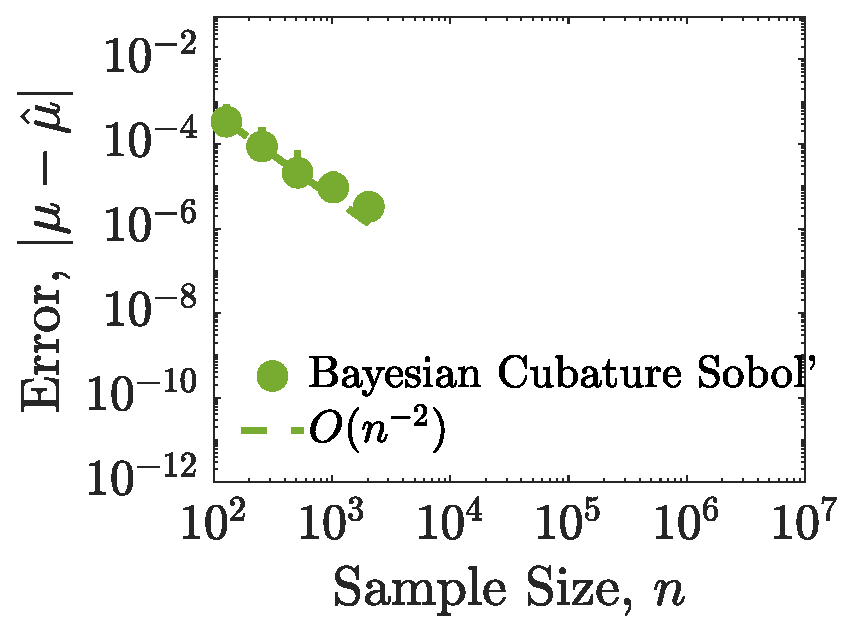
\includegraphics[height=4cm]{MVNBayesianWtSobol}
\end{subfigure}
\centering
\begin{subfigure}[b]{0.49\textwidth}
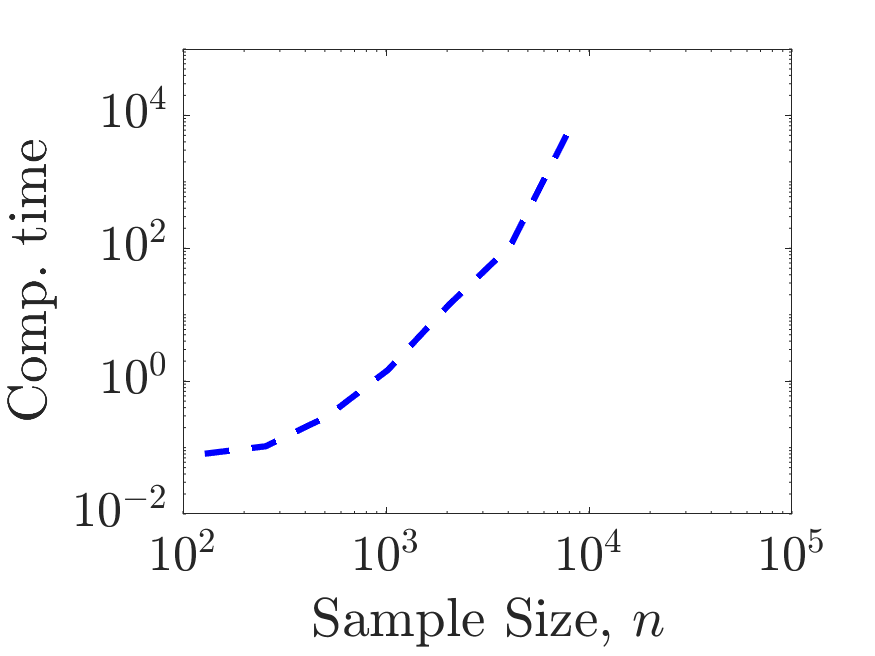
\includegraphics[height=4cm]{MVN_bayesianCubaturecomputeTime}
\end{subfigure}
\caption{MVN for d=2 with Matern kernel  }
\label{fig:MVN_Metern_d2b2}
\end{figure}
On our test computer with Intel i7 3630QM and 16GB RAM memory, it took 118 minutes to compute $\hmu_n$ with $n=2^{13}$. As shown in Figure \ref{fig:MVN_Metern_d2b2}, computation time increases rapidly with $n$. 
Especially, Maximum-likelihood-estimation of $\vtheta$ which needs the loss function, is the most time consuming of all. 
Because the loss functions need to be computed multiple times in every iteration to choose the optimal shape parameter till its minimum is found. 
Not only the complexity increases, also the kernel matrix becomes highly ill-conditioned with increasing $n$ number of data-points.
We must use alternative techniques to overcome this problem.
So, our algorithm in the current form is not straightaway usable for any practical applications.



\section{Fast Automatic Bayesian Cubature}\label{sec:fast_BC}

The generic automatic Bayesian cubature algorithm described in the previous section requires $\Order(n^3)$ operations to estimate $\vtheta$, compute the credible interval width, and compute the cubature.  There is also the potential ill-condtioning that can arise.  This section explains how speed up the calculations and avoid ill-conditioning.  A key is to choose kernels that match the design, $\{\vx_i\}_{i=1}^n$, so that the vector-matrix operations required by Bayesian cubature can be accomplished using fast transforms at a cost of $\Order(n \log(n))$.

\subsection{Fast transform kernel}
We make some assumptions about the relationship between the covariance kernel and the design, which will be shown to hold in Section \ref{sec:shift_invariant_kernel} for rank-1 lattices and shift-invariant kernels.  Firs we introduced the notation
\begin{align}
\nonumber
\mC &= \Big(C_\vtheta(\vx_i,\vx_j)\Big)_{i,j=1}^n  = (\vC_1,...,\vC_n) 
\\
\label{eqn:ftk_factor}
&= \frac 1n \mV \mLambda \mV^H  = \frac 1n \mV^* \mLambda \mV^T , 
\quad \quad \mV^H = n \mV^{-1}, \\
\nonumber
\mCInv  &= \frac 1n \mV \mLambda^{-1} \mV^H
= \frac 1n \mV^* \mLambda^{-1} \mV^T,
\end{align}
where $\mV^H$ is the Hermitian of $\mV$.  The columns of matrix $\mV$ are eigenvectors of $\mC$, and $\mLambda$ is a diagonal matrix of eigenvalues of $\mC$.
\begin{gather*}
\mV = (\vV_1,...,\vV_n)= (\vv_1,...,\vv_n)^T , \; \text{also} \;  \vv_1 = \vV_1 = \vone
\\
\mLambda = \diag(\vlambda), \quad 
\vlambda = (\lambda_1, ... \lambda_n),
\\
\mV^{-1} = \frac 1n \mV^H, \;
\mCInv  = \frac 1n \mV \mLambda^{-1} \mV^H
 = \frac 1n \mV^* \mLambda^{-1} \mV^T.
\end{gather*}
For any $n \times n$ vector $\vb$, define the notation  $\widehat{\vb} := \mV^T \vb$.

We make two assumptions that allow the fast computation:
\begin{subequations} \label{fastcompAssump}
	\begin{gather}
	\mV \text{ may be identified analytically}, \\
	\vv_1 = \vV_1 = \vone, \\
     \mV^T \vb  \text{ requires only $\Order(n \log(n))$ operations } \forall \vb.
	\end{gather}
\end{subequations}
We call the transformation $\vz \mapsto \mV^T \vz$ a \emph{fast transform}.  

Under assumptions \eqref{fastcompAssump} the eigenvalues may be identified as the fast transform of the first column of $\mC$:
\begin{align}
\nonumber
 \vlambda 
 & = \begin{pmatrix}
 \lambda_1 \\ \vdots \\ \lambda_n
 \end{pmatrix} = \mLambda \vone = \mLambda \vv_1 
 = \underbrace{\left( \frac 1n \mV^T  \mV^* \right) }_{\mathsf{I}} \mLambda \vv_1 \\
  &= \mV^T \left( \frac 1n \mV^* \mLambda \vv_1 \right)
 = \mV^T \vC_1 =  \widehat{\vC}_1.
 \label{eqn:fast_transform_to_eigvalues}
\end{align}
Also note that the fast transform of $\vone$ has a simple form
\begin{align}
\widehat{\vone}
& = \mV^T \vone = \mV^T \vV_1^* = \begin{pmatrix}n  \\ 0 \\ \vdots \\ 0 \end{pmatrix}.
\label{eqn:fast_transform_one}
\end{align}

Many of the terms that arise in the calculations in  Algorithm \ref{algorithm1} are of the form $\va^T\mC^{p}\vb$ for integer $p$.  These can be calculated via the transforms $\widehat{\va} = \mV^T \va$ and $\widehat{\vb} = \mV^T \vb$ as 
\begin{equation*}
\va^T\mC^p\vb = \frac 1n \va^T \mV \mLambda^p \mV^H \vb
= \frac 1n \widehat{\va}^T\mLambda^p \widehat{\vb}^*
= \frac 1n \sum_{i=1}^n \lambda_i^p \widehat{a}_i \widehat{b}_i^*, 
\end{equation*}
In particular,
\begin{align*}
\vone^T\mC^{-p}\vone & = \frac{n}{\lambda_1^p},
&
\vone^T\mC^{-p}\vy &= \frac{\widehat{y}_1}{\lambda_1^p},
\\
\vy^T\mC^{-p} \vy &= \frac 1n \sum_{i=1}^n \frac{\abs{\widehat{y_i}}^2}{\lambda_i^p},
\\
\vc^T\mCInv \vone &= \frac{\widehat{c}_1}{\lambda_1},
&
\vc^T\mCInv \vc &= \frac 1n \sum_{i=1}^n \frac{\abs{\widehat{c}_i}^2}{\lambda_i},
\end{align*}
where $\widehat{\vy} = \mV^T \vy$ and 
$\widehat{\vc} = \mV^T \vc$. 

The covariance kernel used in practice also may satisfy an additional assumption:
\begin{equation} \label{addAssump}
\int_{[0,1]^d} C(\vt,\vx) \, \D \vt = 1 \qquad \forall \vx \in [0,1]^d,
\end{equation}
which implies that $c_0 = 1$ and $\vc = \vone$.  Under \eqref{addAssump}, the expressions above may be further simplified:
\begin{equation*}
\vc^T\mCInv \vone =
\vc^T\mCInv \vc = \frac{n}{\lambda_1}.
\end{equation*}


\subsection{Empirical Bayes}

Under assumptions \eqref{fastcompAssump}, the empirical Bayes parameters in \eqref{eqn_m_MLE}, \eqref{eqn_s2_MLE}, \eqref{eqn:thetaMLE} \eqref{eqn:cubMLE}, and \eqref{eqn:errMLE} can be expressed in terms of the fast transforms of the function data, the first column of the Gram matrix, and $\vc$ as follows:
\begin{align}
\nonumber
m_\MLE &=  \frac{\widehat{y}_1}{n} = \frac 1n \sum_{i=1}^n y_i,
\\
\nonumber
s^2_\MLE 
& =
\frac{1}{n^2} 
\sum_{i=2}^n \frac{\abs{\widehat{y}_i}^2}{\lambda_i} \\
\nonumber 
\vtheta_\MLE
&= 
\argmin_{\vtheta}
\left[
\log\left(
\sum_{i=2}^n \frac{\abs{\widehat{y_i}}^2}{\lambda_i}
\right) 
 \right . \\
&
\label{eqn_MLE_loss_func_optimized_2}
\qquad \qquad \qquad \qquad  \left . + 
\frac{1}{n}\sum_{i=1}^n \log(\lambda_i)
\right]
\\
\hmu_\MLE  &= 
\frac{\widehat{y}_1}{n} +
\frac 1n \sum_{i=2}^n \frac{ \widehat{c}_i \widehat{y}_i^*}{\lambda_i} \\
\err_\MLE  &
=
  \frac{2.58}{n}\sqrt{
 \sum_{i=2}^{n} \frac{\abs{\widehat{y}_i}^2}{\lambda_i}  
				\,
				\left( c_0 - \frac 1n \sum_{i=1}^n \frac{\abs{\widehat{c}_i}^2}{\lambda_i} \right) 
			},
\end{align}
Since all the quantities on the right hand sides can be obtained in in $\Order(n \log(n))$ operations by fast transforms, the left hand sides are all computable using the asymptotic computational cost.

Under the further assumption \eqref{addAssump} it follows that 
\begin{align}
\nonumber
\hmu_\MLE  &= 
\frac{\widehat{y}_1}{n} = \frac 1n \sum_{i=1}^n y_i,\\
\err_\MLE  &
=
\frac{2.58}{n}\sqrt{
	\sum_{i=2}^{n} \frac{\abs{\widehat{y}_i}^2}{\lambda_i}  
	\,
	\left( 1 -  \frac{n}{\lambda_1} \right) 
}.
\end{align}
Thus, in this  case $\hmu$ is simply the sample mean.



\subsection{Full Bayes}
For the full Bayes approach the cubature is the same as for empirical Bayes.  We also defer to empirical Bayes to estimate the parameter $\vtheta$.  The width of the confidence interval is $\err_{\textup{full}} 
:= t_{n_j-1,0.995} \hsigma_{\textup{full}}$, where $\hsigma_{\textup{full}}^2$ can also be computed swiftly under assumptions \eqref{fastcompAssump}:
\begin{multline*} %\label{FJH:eq:signmaFull}
\widehat{\sigma}^2_{\textup{full}}
=
\frac{1}{n(n-1)} \sum_{i=2}^n \frac{\abs{\widehat{y_i}}^2}{\lambda_i}
\\
\times
\left[\frac{\lambda_1}{n}{\left(1 - \frac{\widehat{c}_1}{\lambda_1}\right)^2} + \left(c_0  - \frac 1n \sum_{i=1}^n \frac{\abs{\widehat{c}_i}^2}{\lambda_i}\right) \right] .
\end{multline*}
Under assumption \eqref{addAssump} further simplification can be made:
\begin{equation*} %\label{FJH:eq:signmaFull}
\widehat{\sigma}^2_{\textup{full}}
=
\frac{1}{n(n-1)} \sum_{i=2}^n \frac{\abs{\widehat{y_i}}^2}{\lambda_i} \, \left(\frac{\lambda_1}{n}  - 1  \right).
\end{equation*}



\subsection{Generalized Cross-Validation}

GCV yields a different cubature, which nevertheless can also be computed quickly using the fast transform.  Under assumptions \eqref{fastcompAssump}:
\begin{align*}
m_{\textup{GCV}} & = m_\MLE =  \frac{\widehat{y}_1}{n} = \frac 1n \sum_{i=1}^n y_i,\\
 s^2_{\textup{GCV}} & : =  \frac 1{n} \sum_{i=2}^n \frac{\abs{\widehat{y}_i}^2}{\lambda_i^2}  \left [ \sum_{i=1}^n \frac{1}{\lambda_i} \right]^{-1}, \\
\vtheta_{\textup{GCV}} 
&= \argmin_\vtheta \left[ \log \left ( \sum_{i=2}^n \frac{\abs{\widehat{y}_i}^2}{\lambda_i^2} 
\right) -2\log\left( \sum_{i=1}^n \frac{1}{\lambda_i} \right)
\right], \\
\widehat{\mu}_{\textup{GCV}}
&= \hmu_\MLE  = 
\frac 1n \sum_{i=2}^n \frac{ \widehat{c}_i \widehat{y}_i^*}{\lambda_i}, \\
\err_{\textup{GCV}} & =
\frac{2.58}{\sqrt{n}}\left\{\sum_{i=2}^n \frac{\abs{\widehat{y}_i}^2}{\lambda_i^2}  \left [ \sum_{i=1}^n \frac{1}{\lambda_i} \right]^{-1} \right.
\\ 
&\qquad \qquad \left . \times
	\left( c_0 - \frac 1n \sum_{i=1}^n \frac{\abs{\widehat{c}_i}^2}{\lambda_i} \right) 
\right\}^{1/2}.
\end{align*}
Moreover, under further assumption \eqref{addAssump} it follows that 
\begin{align}
\nonumber
\widehat{\mu}_{\textup{GCV}}
&= \hmu_\MLE
\frac{\widehat{y}_1}{n} = \frac 1n \sum_{i=1}^n y_i,\\
\nonumber
\err_{\textup{GCV}} & =
\frac{2.58}{\sqrt{n}}\left\{\sum_{i=2}^n \frac{\abs{\widehat{y}_i}^2}{\lambda_i^2}  \left [ \sum_{i=1}^n \frac{1}{\lambda_i} \right]^{-1} \right.
\\ 
&\qquad \qquad \left . \times
	\left( 1 -  \frac{n}{\lambda_1} \right)  
\right\}^{1/2}.
\end{align}
Thus, in this  case $\hmu$ is simply the sample mean.








\section{Integration Lattices and Shift Invariant Kernels}
\label{sec:shift_invariant_kernel}
We have established the concept of fast transform and showed how it can make the computations faster. But we assumed there exist a kernel that meets the requirements.
Now we are going to show a example.
The following shift invariant kernel satisfies the requirements of the fast transform kernel when combined with Rank-1 lattice points:
\iffalse
\begin{align}
\nonumber
C(\vx, \vt) := & \sum_{\vk \in \mathbb{Z}^d} \alpha_{\vk}  e^{2 \pi\sqrt{-1} \vk^T\vx}
e^{-2 \pi\sqrt{-1} \vk^T\vt} & ,\; \text{where} \; {\alpha}_{\bm{0}} = 1
\\
\nonumber
= & \sum_{\vk \in \mathbb{Z}^d} {\alpha_{\vk}  } 
e^{2 \pi\sqrt{-1} \vk^T(\vx -\vt )}
\end{align}
\fi
\begin{align}
\label{bayes_SI_kernel}
C_\vtheta(\vx, \vt) := &  \sum_{\vk \in \mathbb{Z}^d} \alpha_{\vk,\vtheta}  e^{2 \pi\sqrt{-1} \vk^T\vx}
e^{-2 \pi\sqrt{-1} \vk^T\vt},
\\
\nonumber
\text{where} \quad
\alpha_{\vk,\vtheta} := & \prod_{l=1}^d \frac{1}{\max(\frac{|k_l|}{\theta_l},1)^r_{\theta_l\leq 1}}  \;,  \quad \text{with} \; {\alpha}_{\bm{0},\vtheta} = 1,
\end{align}
where $d$ is number of dimensions and $\alpha_{\vk}$ is a scalar. The Gram matrix formed by this kernel is a Hermitian matrix. 
With some more simplifications:
\begin{align*}
%\label{bayes_SI_kernel_theta}
C_\vtheta(\vx, \vt) = & \prod_{l=1}^d  
\left[ 1 +
\sum_{k_l=1}^\infty
\Big|\frac{\theta_l}{k_l}\Big|^r 
2 \cos({2 \pi\sqrt{-1} k_l(x_l - t_l )})
\right].
\end{align*}

The \textit{shape parameter} $\vtheta$ is used to make the kernel customizable. To be specific, the {shape parameter} tweaks the kernel, so that the function space spanned by the kernel closely resembles the space where the integrand function belongs.

%where $\vtheta$ is the {shape parameter}. 
%The reason for these simplifications will be obvious in the further sections.
This form of the kernel is very convenient to use in any analytical derivations or proofs, but not suitable for use with finite precision computers as this kernel involves infinite sum. It is preferred to have a simpler expression of the kernel without infinite sum for practical computations. 




\subsection{Using Lattice points}
Along with the kernel (\ref{bayes_SI_kernel}), Rank-1 lattice points $\vx_i \in \mathsf{L}_{n,\bm{h}}$ are used to get the \textit{fast transform kernel}. 
In this work, we use the lattice points as defined in \cite{Rank1Lattice}:
\begin{align*}
%\label{eqn:lattice_defn}
\mathsf{L}_{n,\bm{h}} := \lbrace \vx_i :=  \bm{h} \frac{ i-1}{n} \mod 1 ;\ \; i=1,\hdots,n
\rbrace,
\end{align*}
Where $\bm{h}$ is the generating vector.
Its dual lattice is defined as:
\begin{align*}
%\label{eqn:dual_lattice}
\mathsf{L}_{n,\bm{h}}^{\perp } := 
\lbrace 
\vk \in \mathbb{Z}^d : \vh^T \vk \equiv 0 \;\;  (\mod n)
\rbrace,
\end{align*}


\begin{figure}[htp]
\centering
    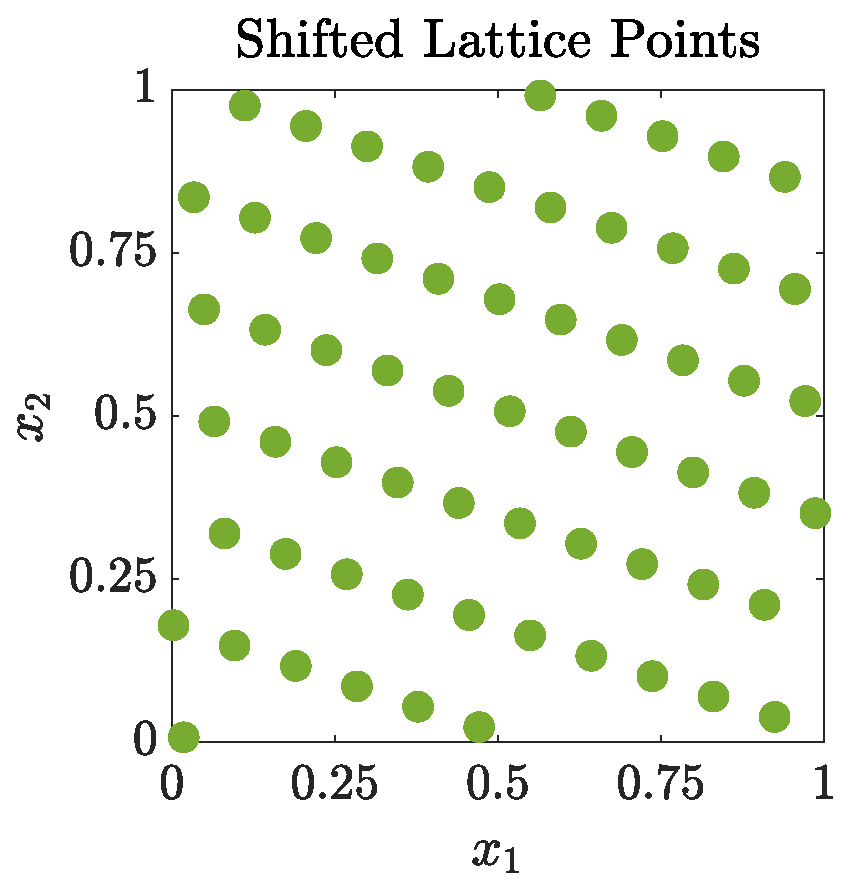
\includegraphics[height=5cm]{ShiftedLatticePoints}
    \caption{Randomly shifted Lattice points in d=2  }
\end{figure}


With lattice points, the kernel is written as:
\begin{align*}
C(\vx_i, \vx_j)
 &=
\sum_{\vk \in \mathbb{Z}^d} \alpha_{\vk}  
e^{ 2 \pi\sqrt{-1} \vk^T  \frac{\bm{h} i}{n}}
e^{-2 \pi\sqrt{-1} \vk^T  \frac{\bm{h} j}{n}}
\\
 &=
\sum_{\vk \in \mathbb{Z}^d} \alpha_{\vk}  
e^{2 \pi\sqrt{-1} \vk^T \bm{h} \frac{(i-j)}{n}}
\end{align*}
Please note that `$\mod 1$' need not be used explicitly in $C(\vx_i, \vx_j)$ since 
$
e^{\pm 2 \pi \sqrt{-1}} = 1
$. 
The kernel (\ref{bayes_SI_kernel}), when used with Rank-1 Lattice points, leads to symmetric and circulant Gram matrix $\mC$.
We can demonstrate the resulting Gram matrix satisfies the conditions of a fast transform. 


\subsection{Computing the kernel using Bernoulli polynomials}
The shift-invariant-kernel (\ref{bayes_SI_kernel}) cannot be computed directly due to it's  infinite sum. 
If the coefficients $\alpha_{\vk}$ were chosen appropriately, then there exist a direct expression for the kernel in terms of Bernoulli polynomial. 
We can use the Fourier series expansion properties \cite{DLMF} of Bernoulli polynomial $B_r$ to find the appropriate $\alpha_{\vk}$. This provides a closed form expression for the kernel without the infinite sum. It also allows to choose the smoothness of kernel, i.e, how fast the coefficients $\alpha_{\vk}$ in (\ref{bayes_SI_kernel}) decay.
The following very useful expansion is referenced from \cite{DLMF} under eqn (24.8.3):
\begin{multline}
\label{dlmf_bernoulli_24_8_3}
B_{r}(x) = \frac{-r!}{(2 \pi \sqrt{-1})^{r}} 
\sum_{\substack{k \neq 0,\\ k=-\infty}}^\infty 
\frac{e^{2\pi\sqrt{-1} k x}}{k^{r}}
\;\;
\\
\begin{cases}
\text{for} \;\; r=1, \qquad \; 0 < x < 1 \\
\text{for} \;\; r=2,3,\hdots \;\; 0 \leq x \leq 1
\end{cases}
\end{multline}

Our goal is to replace the infinite sum of the kernel using Bernoulli polynomials. This would allows the computations to be carried out in any software like Matlab.
For 1-D $(d=1)$ rewriting (\ref{dlmf_bernoulli_24_8_3}):
\begin{multline*}
\sum_{k \neq 0, k=-\infty}^\infty \frac{e^{2\pi\sqrt{-1} k |x|}}{ (\frac{k}{\theta})^{r}}
\\
=
-{\theta^r} B_{r}(|x|) \frac{(2 \pi \sqrt{-1})^{r}}{r!}
\; \text{for} \; -1 \leq x \leq 1
\end{multline*}
Comparing this expansion with (\ref{bayes_SI_kernel}), one can deduce, for $d=1$:
\[
C({x}, {t}) = 
\alpha_0 + \sum_{k \neq 0, k=-\infty}^\infty \alpha_k e^{2\pi\sqrt{-1} k |x-t|}   
, \; -1 \leq x,t \leq 1,
\]
Where the kernel coefficients ${\alpha}_{\vk}$ can be expressed explicitly:
\[
\alpha_k = 
\begin{cases}
1, & k=0 \\
\frac{1}{k^r}, & \text{otherwise}
\end{cases},
\]
In general for $d>1$, the coefficients $\alpha_{\vk}$ for $C_{\vtheta}(\vx,\vt)$ is computed using:
\begin{align*}
%\label{bayes_kernel_lambda}
\alpha_{\vk, \vtheta} = \frac{1}{\prod_{l=1}^d \max(\frac{|k_l|}{\theta_l}, 1)^r} \; ,
\end{align*}
Where $\vtheta$ is the shape parameter and `$r$' is the Bernoulli polynomial. The value of '$r$' will be chosen specific to the integrand when using in the cubature algorithm. We keep the value of `$r$' to be even positive integer in this work.
Using the above-found results, we get the simplified form of the kernel:
\begin{multline}
\label{the_kernel_eqn_bernoulli}
C_\vtheta(\vx, \vt) =
 \prod_{l=1}^d
1 - \theta_l^r \frac{(2 \pi \sqrt{-1})^{r}}{r!} B_{r}( |{x_l-t_l}| ),
\\
\text{where} \; 0 \leq |x_l - t_l| \leq 1,
\end{multline}
where $\vtheta \in (0,1]^d$ is the {shape parameter}, `$r$' is the order of the Bernoulli polynomial $B_{r}$.

We call \eqref{the_kernel_eqn_bernoulli} a Fourier kernel as the resulting Fast transform is the \emph{Fast Fourier transform} (FFT). Plots of this kernel in $d=2$ is shown in \figref{fig:Fourier_kernel}.







\begin{figure}
	\centering
	\begin{subfigure}{0.40\textwidth}
		\includegraphics[width=\textwidth]{"fourier_kernel r_2 shape_10by100"}
	\end{subfigure}
	\centering
	\begin{subfigure}{0.40\textwidth}
		\includegraphics[width=\textwidth]{"fourier_kernel r_2 shape_90by100"}
	\end{subfigure}
	\centering
	\begin{subfigure}{0.40\textwidth}
		\includegraphics[width=\textwidth]{"fourier_kernel r_4 shape_10by100"}
	\end{subfigure}
	\centering
	\begin{subfigure}{0.40\textwidth}
		\includegraphics[width=\textwidth]{"fourier_kernel r_4 shape_90by100"}
	\end{subfigure}
\caption{Fourier kernel \eqref{the_kernel_eqn_bernoulli} with $r=2,4$ and $\theta = 0.1, 0.9$}
\label{fig:Fourier_kernel}
\end{figure}








\subsection{Eigenvalues and Eigenvectors of $\mC$}

The kernel's Gram matrix $\mC$ is circulant. It is generated by the vector:
\begin{equation}
\label{eqn_top_row_of_kernel_matrix}
\left( \vCvtheta(\vx_1,\vx_1),\vCvtheta(\vx_2,\vx_1),...,\vCvtheta(\vx_{n},\vx_1 \right) 
)^T =: \vC_1,
\end{equation}
Which is the first row or column of $\mC$ (since it is a symmetric matrix).  By the properties of circulant matrix, the normalized eigenvectors are:
\begin{multline*}
%\label{eqn_eig_vectors_of_mC}
\left(
1, 
e^{- 2 \pi \sqrt{-1} \frac{j}{n}},
e^{- 2 \pi \sqrt{-1} \frac{2j}{n}}
,...,
e^{- 2 \pi \sqrt{-1} \frac{j(n-1)}{n}}  
\right)^T, \\ \text{for} \;
j=0,1,...,n-1 .
\end{multline*}

The matrix constructed with these eigenvectors is: 
\begin{align*}
\mV  := \left(e^{- 2 \pi \sqrt{-1} \frac{i j}{n}} \right)_{i,j=0}^{n-1},\;
\mV^H := \frac{1}{n} \left(e^{ 2 \pi \sqrt{-1} \frac{i j}{n}} \right)_{i,j=0}^{n-1},
\end{align*}
Where the first column of $\mV$, $\vV_1 = \vone$.
The columns of $\mV$ are complex exponential vectors independent of the kernel values. But their corresponding eigenvalues are:
\begin{align*}
%\label{eqn_eig_values_of_mC}
\mLambda = \left( \lambda_j \right)_{j=1}^{n} = \mV^T \vC_1 := \mathcal{DFT} \left\lbrace \vC_1 \right\rbrace,
\end{align*}
i.e., eigenvalues of the matrix $\mC$ are computed by applying DFT over $\vC_1$. 
for this kernel, the corresponding fast transform is \emph{Fast Fourier Transform} (FFT). 
The kernel's Gram matrix $\mC$ can be written in the factorized form:
\begin{align*}
\mC = \frac1n \mV \mLambda \mV^H,
\end{align*}
This is the exact factorization used for the construction of fast transform. 
Another requirement $\vV_1 = \vone$ is also met.
Additionally, computational cost of FFT is $\Order(n \log n)$.
Thus we can conclude the shift invariant kernel in eqn (\ref{bayes_SI_kernel}), obeys all the requirements to be considered as a {fast transform kernel}. So the operation $\mV^T z$ is a fast transform.
Numerical experiments using this kernel will be shown in the section (\ref{sec:numerical_experiments}).






\subsection{Additional assumptions}
The shift invariant kernel (\ref{bayes_SI_kernel}) has some more desirable properties, leading to $c_0=1$ and $\vc = \vone$, which will help to make the computations even faster:
\begin{multline*}
%\label{eqn:ftk_integral_definitions}
\displaystyle
c_0 =\int_{[0,1]^d\times [0,1]^d}C_\vtheta(\vx,\vt) \dvx \dvt = 1, 
\\
\quad \vc = \left( \int_{[0,1]^d}C_\vtheta(\vx_i,\vt) \dvt\right)_{i=1}^n = \vone .
\end{multline*}

This gives simplified error bound:
\begin{align*}
\errn &=
2.58\sqrt{
\frac {1}{n^2} \sum_{i=2}^{n} \frac{\abs{\widehat{y}_i}^2}{\lambda_i}  
\,
\left( c_0 - \frac 1n \sum_{i=1}^n \frac{\abs{\widehat{c}_i}^2}{\lambda_i} \right) 
}, 
\\
&= 
2.58\sqrt{
\frac {1}{n^2} \sum_{i=2}^{n} \frac{\abs{\widehat{y}_i}^2}{\lambda_i}  
\,
\left( 1 - \frac{n}{\lambda_1}  \right) 
}, 
\\
& \text{where} \quad \widehat{\vc} = (n,0,...,0)^T, \quad 
\widehat{\vy} = \mV^T \vy,  
\widehat{\vc} = \mV^T \vc. 
\end{align*}


And the cubature:
\begin{align*}
\nonumber
\hmu_n(f) &= w_0 + \vw^T \vy 
= 
\frac{\widehat{y}_1}{n} +
\frac 1n \sum_{i=2}^n \frac{ \widehat{c}_i \widehat{y}_i^*}{\lambda_i} \\
& = \frac{\widehat{y}_1}{n}, \quad \text{since} \quad
 \widehat{\vc}_i=0 \; \forall \; i \neq 0
\end{align*}





\subsubsection{Full Bayes}
Final version of full Bayes equations optimized using the properties of the shift invariant kernel are:
\begin{align}
\label{FJH:eq:cubFull}
\widehat{\mu}_{\textup{full}}  \vert ( \vf = \vy) &= 
 \frac{\widehat{y}_1}{n} ,
\end{align}
\begin{align}
\vtheta_{\textup{GCV}} 
&= \argmin_\vtheta \left[ \log \left ( \frac 1n \sum_{i=2}^n \frac{\abs{\widehat{y}_i}^2}{\lambda_i^2} 
\right) -2\log\left( \sum_{i=1}^n \frac{1}{\lambda_i} \right)
\right]
\end{align}
\begin{multline*}
%\label{FJH:eq:signmaFull}
\widehat{\sigma}^2_{\textup{full}}  \vert ( \vf = \vy) 
= 
\frac{1}{n-1} 
\frac{1}{n} \sum_{i=2}^n \frac{\abs{\widehat{y_i}}^2}{\lambda_i} \times
\\
\qquad \qquad \left[\frac{\lambda_1}{n}{\left(1 - \frac{\widehat{c}_1}{\lambda_1}\right)^2} + \left(c_0  - \frac 1n \sum_{i=1}^n \frac{\abs{\widehat{c}_i}^2}{\lambda_i}\right) \right] 
\\
= 
\frac{1}{n-1} 
\frac{1}{n} \sum_{i=2}^n \frac{\abs{\widehat{y_i}}^2}{\lambda_i} 
\times
\left( 1- \frac{n}{\lambda_1}\right) \left[\frac{\lambda_1}{n}{\left(1 - \frac{n}{\lambda_1}\right)} + 1\right] 
\\
= 
\frac{1}{n(n-1)} \sum_{i=2}^n \frac{\abs{\widehat{y_i}}^2}{\lambda_i}
\times
\left( \frac{\lambda_1}{n} - 1\right)  
\end{multline*}

The stopping criterion for the full Bayes case,  
\begin{multline} \label{FJH:eq:stopcritHyper}
n  = \min \biggl \{n_j \in \posIntegers:  
\\
\frac {t_{n_j-1,0.995}^2}{n_j(n_j - 1)} 
\left( \frac{\lambda_1}{n_j} - 1\right)  
\times
 \sum_{i=2}^{n_j} \frac{\abs{\widehat{y_i}}^2}{\lambda_i}  \le \varepsilon^2 \biggr\}.
\end{multline}



\subsection{Variable transforms}
Fast transform kernel technique discussed with shift invariant kernel eqn(\ref{bayes_SI_kernel}) and lattice points so far, assumes the integrand is periodic and has continuous derivatives on the boundaries of the domain $[0,1]^d$. Non-periodic functions do not live in the space spanned by the kernel.
Variable transformation or periodization transform techniques are typically used to improve the accuracy in multi-dimensional numerical integrations where boundary conditions needs to be enforced. These transformations could be either polynomial, exponential and also trigonometric nature.
\begin{align*}
\text{Baker's} & : \tilde{f}(\vt) 
= f\left( \left(1-2 \abs{t_j-\frac{1}{2}} \right)_{j=1}^d \right) 
\\
\text{C0} & : \tilde{f}(\vt) 
= f\left( \vg_0 \right)\prod_{j=1}^d g'_0(t_j), 
  \; \vg_0 = \left( g_0(t_j) \right)_{j=1}^d
\\
\text{C1} & : \tilde{f}(\vt) 
= f\left( \vg_1\right)\prod_{j=1}^d g'_1(t_j),
  \; \vg_1 = \left( g_1(t_j) \right)_{j=1}^d 
\\
\text{Sidi's C1} & : \tilde{f}(\vt) 
= f\left( \bm{\psi}_2 \right) \prod_{j=1}^d \psi'_2(t_j),
  \; \bm{\psi}_2 = \left( {\psi}_2(t_j) \right)_{j=1}^d
\\
\text{Sidi's C2} & : \tilde{f}(\vt) 
= f\left( \bm{\psi}_3 \right) \prod_{j=1}^d \psi'_3(t_j),
  \; \bm{\psi}_3 = \left( {\psi}_3(t_j) \right)_{j=1}^d
\end{align*}
where
\begin{multline*}
g_0(t) = 3 t^2 - 2 t^3,   g'_0(t) = 6t(1-t))
\\
g_1(t) = t^3(10-15t+6t^2),   g'_1(t) = 30t^2(1-t)^2
\\
\psi_2(t) = 
\left(t - \frac{1}{2\pi} \sin(2\pi t) \right) 
,  \psi'_2(t) = 
\left(1 - \cos(2 \pi t)  \right) 
\\
\psi_3(t) = 
\frac{1}{16} \left(8-9\cos(\pi t)+ \cos(3\pi t) \right) 
, 
\\ 
\psi'_3(t) = 
\frac{1}{16} \left(9 \sin(\pi t) \pi - \sin(3 \pi t) 3 \pi \right) 
\end{multline*}

These transforms vary in terms of computational complexity and accuracy, shall be chosen on a need basis.
Such as:
\begin{enumerate}
\item Baker's : Baker's transform or called tent map in each coordinate. It preserves only continuity but it is easier to compute.
\item C0 : Polynomial transformation only ensures periodicity of function.
\item C1 : Polynomial transformation preserving the first derivative.
\item C1sin : Sidi's transform with Sine, preserving the first derivative. This is, in general, a better option than `C1'.
\item C2sin : Sidi's transform with Sine, preserving upto second derivative. We use this when smoothness of `C1sin' is not sufficient and need to preserve upto second derivative.
\end{enumerate}






\subsection{Iterative Discrete Fourier transform for function values}

Automatic cubature algorithms needs to compute Discrete Fourier transform of function values $\vy = \left(f(\vx_i)\right)_{i=1}^n$ in every iteration with newly added points. Recomputing the whole Fourier transform in every iteration can be avoided when using Rank-1 Lattice points by using structural properties of the Lattice points.  
Discrete Fourier transform is defined as :
\begin{align*}
\mathcal{DFT} \{y \} := \hat{y} = \left( \sum_{j=1}^{n} y_j 
e^{-\frac{2\pi \sqrt{-1}}{n} (j-1) (i-1) }
\right)_{i=1}^{n}
\end{align*}
In essence:
\begin{align*}
\hat{y}_i &=  \sum_{j=1}^{n} y_j 
e^{- \frac{2\pi \sqrt{-1}}{n} (j-1) (i-1) }
\end{align*}
We could rearrange the sum into even indexed $j=2l$ and odd indexed $j=2 l + 1$:

\begin{multline*}
\hat{y}_i =  
\underbrace{
\sum_{l=1}^{n/2} y_{2l} 
e^{- \frac{2\pi \sqrt{-1}}{n/2} (l-1)( i-1) }
}_{\text{DFT of even-indexed part of}\; y_i}
\\
+
e^{- \frac{2\pi \sqrt{-1}}{n} (i-1) }
\underbrace{
\sum_{l=1}^{n/2} y_{2l+1} 
e^{- \frac{2\pi \sqrt{-1}}{n/2} (l-1)( i-1) }
}_{\text{DFT of odd-indexed part of}\; y_i},
\end{multline*}
Which shows two separately computed DFTs can be combined to produce single output. For example, the odd indexed were the existing DFT and the even indexed are from the new halve of samples, algorithm wants to add to improve accuracy.
We use this concept to avoid recomputing the full length DFT of $\vy$ in every iteration. In other words, DFT is computed only for the newly added samples in every iteration.















\subsection{Overcoming the cancellation error}
During the numerical experiments, we noticed numerical cancellation error in the computation of the term, especially for the bigger values $n > 2^{15}$. Cancellation error happens because two almost equal values are subtracted, when they differ only in very high decimal values. 
\[
\left(c_{0,\vtheta} - {\vc}_{\vtheta}^T\mCInv\vc_{\vtheta} \right) = 
\left(
1 - \frac{n }{\lambda_1} \right)
\]
In this expression $\frac{n}{\lambda_1}$ almost close to $1$.
We would like to explore techniques to avoid the subtraction in this computation.
Let's recollect the definition of the shift invariant kernel:
\begin{align*}
C(\vx_i, \vx_j) = \prod_{k=1}^d \left[1 + \theta B(\{x_{i_k} - x_{j_k}\}) \right].
\end{align*}
Let's define the modified kernel:
\begin{align*}
\widetilde{C}(\vx_i, \vx_j) &:= C(\vx_i, \vx_j) - 1,
\\
\text{Then Its Gram matrix:} \quad \tmC &= \mC - \vone \vone^T,
\end{align*}
Let $(\lambda_1, ..., \lambda_n)$ be the eigenvalues of $\mC$. Similarly let $(\tlambda_1, ..., \tlambda_n)$ be the eigenvalues of $\tmC$. As per the definition of the Gram matrix $\mC$, the eigenvector corresponding to $\lambda_1$ is a vector one $\vone$. 
Then:
\begin{equation}
\nonumber
\lambda_1 \vone  = \mC \vone 
 = (\tmC + \vone \vone^T) \vone
 = \tlambda_1 \vone + n \vone,
\end{equation}
This shows $\tlambda_1 = \lambda - n$. In fact for the rest of the values are:
\begin{align}
\label{eqn:lambda_to_tlambda_relation}
\tlambda_j = \lambda_j, \; \forall j=1,...,n-1.
\end{align}

Let $\vv_j, \forall j=0,...,n-1$ be the eigenvectors of $\mC$, similarly
 $\tvv_j, \forall j=0,...,n-1$ be the eigenvectors of $\tmC$,
\begin{align*}
\vv_j^T \mC \vone = \lambda_1 \vv_j^T \vone
 = \vone^T \mC \vv_j
 = \lambda_j \vone^T  \vv_j
 \end{align*}
Since $\lambda_1 \neq \lambda_j$, the above statement implies $\vv_j^T \vone = 0$. This interesting property provides the proof of the eqn. (\ref{eqn:lambda_to_tlambda_relation}).
\[
\lambda_j \vv_j = \mC \vv_j = \mathsf{1}_{n \times n} \vv_j + \tmC \vv_j 
= \tmC \vv_j = \tlambda_j \vv_j ,
\]
Thus proven. 
Using this result, 
cancellation error in the computation of $\errn$ can be avoided:
\begin{align*}
\left( 1 - \frac{n }{\lambda_1} \right) 
& = \left( 1 - \frac{n }{\tlambda_1 + n} \right)
\\
& = \left( \frac{\tlambda_1 + n - n }{\tlambda_1 + n} \right)
 = \left( \frac{\tlambda_1 }{\tlambda_1 + n} \right).
\end{align*}


The following technique shows an iterative approach to compute $\tilde{C}(\vx_i,\vx_j)$ for $d > 1$. This iterative technique is developed using induction:
\begin{align*}
d=1 &:& C_1 &= 1 + \theta B(\{x_{i_1} - x_{j_1}\}) = 1 + \tilde{C}_1
\\
d=2 &:& C_2 &= [1 + \theta B(\{x_{i_2} - x_{j_2}\})] [1 + \tilde{C}_1]
\\
    &&      &= 1 +  \theta B(\{x_{i_2} - x_{j_2}\}) [1 + \tilde{C}_1]  +  \tilde{C}_1 
\\
    &&      &= 1 +  \underbrace{\theta B(\{x_{i_2} - x_{j_2}\}) C_1  +  \tilde{C}_1 }_{\tilde{C}_2}
\\
d=3 &&  C_3 &= [1 +  \theta B(\{x_{i_3} - x_{j_3}\})][ 1 + \tilde{C}_2] 
\\
    &&      &= 1 +  \theta B(\{x_{i_3} - x_{j_3}\})[1 + \tilde{C}_2] + \tilde{C}_2
\\
    &&      &= 1 +  \theta B(\{x_{i_3} - x_{j_3}\})C_2 + \tilde{C}_2
\\
\vdots
\\
\forall d>2 && C_d &= [1 +  \theta B(\{x_{i_d} - x_{j_d}\})][ 1 + \tilde{C}_{d-1}] 
\\
&& &= 1 +  \theta B(\{x_{i_d} - x_{j_d}\})[ 1 + \tilde{C}_{d-1}] + \tilde{C}_{d-1}
\\
&& &= 1 +  \theta B(\{x_{i_d} - x_{j_d}\})C_{d-1} + \tilde{C}_{d-1}
\end{align*}














\subsection{Validating Gaussian process assumption}


We begin developing the Bayesian cubature with the assumption that the integrand arises from a Gaussian process. How can we check if $m, s, \vtheta$ and $\mC$ are chosen appropriately so that the $\vf$ is a draw from the Gaussian process?. Here is an attempt to validate that assumption. Let,
\begin{multline*}
\vf = \left( f(\vx_i) \right)_{i=1}^n
\sim \calN \left( m\vone, \mC \right), 
\\
\quad \text{where}\quad \mC = \frac 1n \mV \mLambda \mV^H, \quad \mV^H \mV = n
\end{multline*}
Then,
\begin{align*}
\Ex\left[ \frac{1}{\sqrt{n}} \mLambda^{-\frac 12} \mV^H \vf \right]
& =
\frac{1}{\sqrt{n}} \mLambda^{-\frac 12} \mV^H \Ex[\vf] 
\\
& =
\frac{1}{\sqrt{n}} \mLambda^{-\frac 12} \mV^H m \vone
\\
& = m \sqrt{\frac{n}{\lambda_1}} \left( 
\begin{array}{c}
1 \\ 0 \\ \vdots \\ 0
\end{array}
\right),
\end{align*}
Let $\vf' = \frac{1}{\sqrt{n}} \mLambda^{-\frac 12} \mV^H \vf$,
\begin{align*}
\cov \left[ \vf'  \right]
&=
\frac{1}{n} \Ex\left[  
\mLambda^{-\frac 12} \mV^H (\vf - m \vone)
(\vf - m \vone)^T \mV \mLambda^{-\frac 12}
\right]
\\
&=
\frac{1}{n} \mLambda^{-\frac 12} \mV^H 
\Ex\left[ (\vf - m \vone)
(\vf - m \vone)^T \right] \mV \mLambda^{-\frac 12}
\\
&=
\frac{1}{n} \mLambda^{-\frac 12} \mV^H 
\frac 1n \mV \mLambda \mV^H \mV \mLambda^{-\frac 12}
\\
& = \mathsf{I}
\end{align*}
Thus
\begin{align*}
\vf' \sim \calN \left( 
m' \bm{e}_1,
\mathsf{I}
\right),
\end{align*}
Where $m' = m \sqrt{\frac{n}{\lambda_1}} $.
If we can verify the sample distribution of $\vf'$ is approximately $\calN\left( m' \bm{e}_1, \mathsf{I} \right)$ by using Normal plots, could validate our assumption.

We plotted the Normal plots of $\vf'$ for Keister and Multivariate Normal functions as shown in \figref{fig:mvn-normplot} and \figref{fig:keister-normplot}. These plots show the transformed $\vf'$ follows approximately standard normal with a constant mean.




\begin{figure}
	\centering
	\includegraphics[width=0.9\linewidth]{"figures/arbMean/Keister/C1sin/Keister Normplot d_2 bernoulli_2 Period_C1sin n_32768"}
	\caption{Normal plot : Keister function with arbMean assumption}
	\label{fig:keister-normplot}
\end{figure}




\begin{figure}
	\centering
	\includegraphics[width=0.9\linewidth]{"figures/arbMean/MVN/C1sin/MVN Normplot d_2 bernoulli_2 Period_C1sin n_32768"}
	\caption{Normal plot : MVN with arbMean assumption}
	\label{fig:mvn-normplot}
\end{figure}



















\subsection{Numerical Experiments}
\label{sec:numerical_experiments}

Having all the tools and optimization done handy, now we shall run the numerical simulations to see the performance.

\subsubsection{Test Functions}

The following test functions were used to test the integration speed and accuracy of \textit{Fast Bayesian cubature algorithm} that we developed so far

\begin{enumerate}
\item Exponential of Cosine: 

This is a very simple function, serves as an example to check the working of the cubature,
\begin{figure}
	\centering
	\includegraphics[width=0.95\linewidth]{"figures/ExpCos"}
	\caption[Exp(Cos):]{Exp(Cos) in d=2}
	\label{fig:ExpCos}
\end{figure}
where the function is defined as
\begin{multline*}
f(\vx) = e^{\sum_{i=1}^d\cos(2 \pi x_d)},  
\quad
\int_{[0,1]^d} f(\vx) \dvx = \text{BesselI(0,1)}^d
\end{multline*}
where `$\text{BesselI}$' is the \textit{modified Bessel} function. Exp(Cos) function is periodic in $[0,1]$, so we do not need to use any \textit{transform} to make it periodic.







\item Keister function

The following multidimensional integral example is based on the paper \cite{KeisterExample}, inspired by a physics application.
\begin{figure}
	\centering
	\includegraphics[width=0.95\linewidth]{"figures/Keister_wholeR"}
	\caption[Guaranteed:]{Keister function in d=2}
	\label{fig:keister-R}
\end{figure}

\begin{figure}
	\centering
	\includegraphics[width=0.95\linewidth]{"figures/Keister_cube_0_1"}
	\caption[Guaranteed:]{Keister function transformed to $[0,1]^2$}
	\label{fig:keister-0_1}
\end{figure}


\begin{multline*}
f(\vx) =  \cos(\norm{ \vx}) \exp(-\norm{ \vx }^2) \dvx, \;  
\\
\int_{\reals^d} f(\vx) \dvx  = \frac{2 \pi^{\frac d2}}{\Gamma(\frac d2)} \text{CI}(d), \quad d=1,2,3,\hdots
\\
\text{where}, \Gamma  := \text{gamma function}, \; \text{and}
\\
\text{CI}(1) = \frac{\sqrt{\pi}}{2 \exp(1/4)}, 
\\
\text{SI}(1) = \int_{x=0}^\infty \exp(-\vx^T\vx)\sin(\vx) \dvx 
\\
\qquad =  0.4244363835020225,
\\
\text{CI}(2) = \frac{1-\text{SI}(1)}{2}, \;
\text{SI}(2) = \frac{\text{CI}(1)}{2}
\\
\text{CI}(j) = \frac{(j-2)\text{CI}(j-2)-\text{SI}(j-1)}{2},
\; j =3,4,\hdots
\\
\text{SI}(j) = \frac{(j-2)\text{SI}(j-2)-\text{CI}(j-1)}{2},
\; j =3,4,\hdots.
% ref: https://www.mathworks.com/help/matlab/ref/gamma.html
\end{multline*}












\item Multivariate Normal:


We use the Genz's method to compute Multivariate normal probability as explained below. This method reduces the original dimension of the problem by 1.


\begin{figure}
\centering
\captionsetup[subfigure]{labelformat=empty}
\begin{subfigure}{0.48\textwidth}
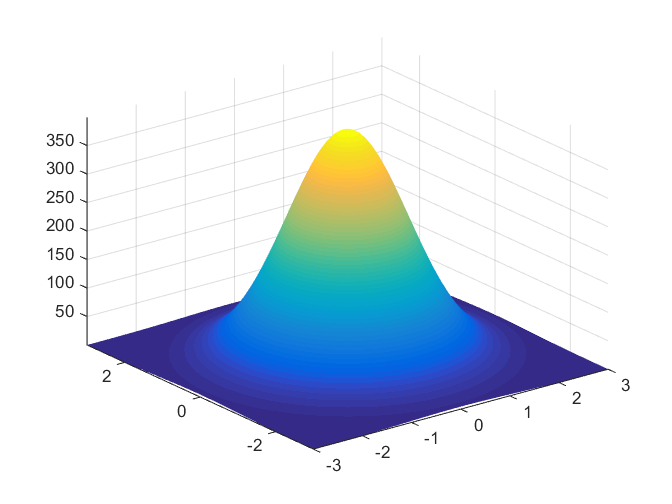
\includegraphics[width=\textwidth]{Plotting_gaussian}
\end{subfigure}
\centering
\begin{subfigure}{0.48\textwidth}

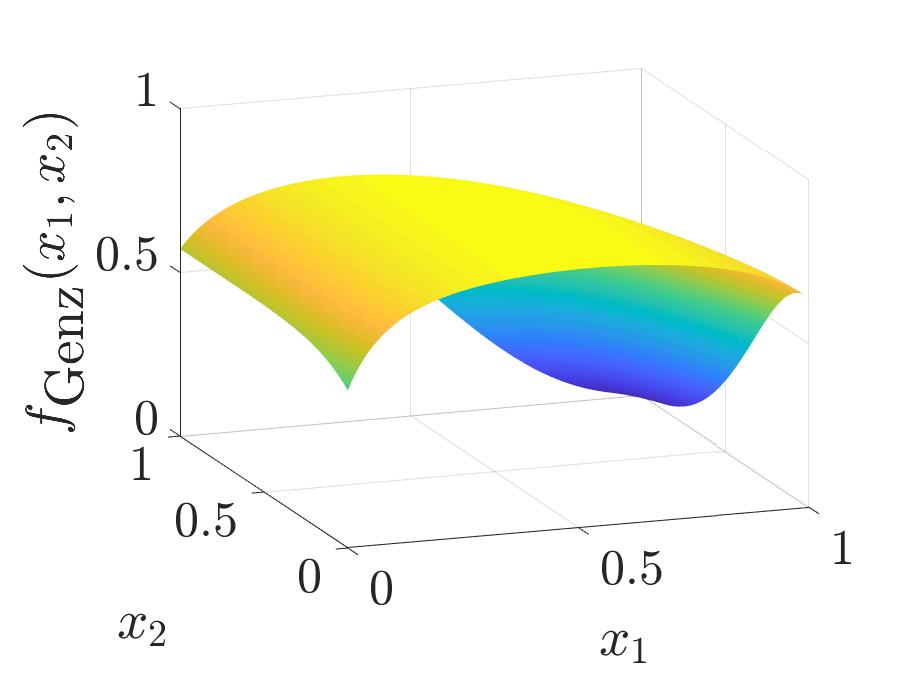
\includegraphics[width=\textwidth]{GenzFun}
\end{subfigure}
\caption{Mutivariate Normal and Genz function }
\label{fig:MVN and Genz}
\end{figure}

\begin{multline*}
\mu = \int_{[\va,\vb] \in \reals^d} \frac{\exp\bigl(- \frac 12 \vt^T \mSigma^{-1} \vt \bigr)}{\sqrt{(2 \pi)^d \det(\mSigma)}} \, \dvt 
\\
\overset{\text{\small\cite{Gen93}}}{=} \,
\int_{[0,1]^{d-1}} f_{\text{Genz}}(\vx) \, \dvx 
\end{multline*} 

where $\mSigma= \mL \mL^T$ is the Cholesky decomposition of the covariance matrix, $\mL = (l_{jk})_{j,k=1}^d$ is a lower triangular matrix, and

\begin{multline*}
\valpha_1 = \Phi(a_1), \qquad \vbeta_1 = \Phi(b_1)
\\
\valpha_j(x_1,...,x_{j-1}) = 
\\
\Phi
\left(
\frac{1}{l_{jj}} 
\left(
a_j - \sum_{k=1}^{j-1} l_{jk} \Phi^{-1}(\valpha_k + x_k(\vbeta_k-\valpha_k))
\right)
\right), 
\\
\qquad \qquad \qquad j=2,...,d,
\\
\vbeta_j(x_1,...,x_{j-1}) = 
\\
\Phi
\left(
\frac{1}{l_{jj}} 
\left(
b_j - \sum_{k=1}^{j-1} l_{jk} \Phi^{-1}(\valpha_k + x_k(\vbeta_k-\valpha_k))
\right)
\right), 
\\
\qquad \qquad \qquad j=2,...,d,
\\
f_{\text{Genz}}(\vx) = \prod_{j=1}^d [\vbeta_j(\vx) - \valpha_j(\vx)]. \hspace{12ex}
\end{multline*}

As we see from the figure, Genz function is not periodic, So we need to make it periodic to get the best accuracy with Bayesian cubature.


We use the following parameter values for the numerical examples
\begin{equation*}
\begin{array}{c|ccc}
 & a  & b & L  \\
\hline
d=2 
 & 
\begin{pmatrix}
-6 \\ -2 \\ -2
\end{pmatrix}
 & 
\begin{pmatrix}
5 \\ 2 \\ 1
\end{pmatrix} 
 & 
\begin{pmatrix}
4 & 1 & 1 \\ 0 & 1 & 0.5 \\ 0 & 0 & 0.25
\end{pmatrix} 
\\
d=3
 & 
\begin{pmatrix}
-6 \\ -2 \\ -2 \\ 2
\end{pmatrix}
 & 
\begin{pmatrix}
5 \\ 2 \\ 1 \\2
\end{pmatrix} 
 & 
\begin{pmatrix}
4 & 1 & 1 & 1\\ 0 & 1 & 0.5 & 0.5 \\ 0 & 0 & 0.25 & 0.25 \\ 0 & 0 & 0 & 0.25
\end{pmatrix} 
\end{array}
\end{equation*}

%\begin{equation*}
%\begin{array}{ccccc}







\item Option pricing

The price of financial derivatives can often be modeled by high dimensional integrals. If the underlying asset is described in terms of a Brownian motion, B, at time $t_1,...,t_d$, then $Z = (B(t_1), ..., B(t_d)) \sim \calN(\vzero,\mSigma)$, where $\mSigma = \left(\min(t_j,t_k) \right)_{j,k=1}^d$, and the fair price of the option is:
\begin{align*}
\mu = \int_{\reals^d} \text{payoff}(\vz) \frac{\exp(\frac 12 \vz^T\mSigma^{-1}\vz)}{\sqrt{(2\pi)^d \det(\mSigma)}} \dvz = \int_{[0,1]^d} f(\vx) \dvx
\end{align*}
where the function {payoff(.)} defines the discounted payoff of the option,
\begin{align*}
f(\vx) = \text{payoff}(\vz), & \quad \vz = \mL 
\begin{pmatrix}
\Phi^{-1}(x_1) \\ \vdots \\ \Phi^{-1}(x_d)
\end{pmatrix},
\end{align*}
and $\mL$ is any square matrix satisfying $\mSigma = \mL \mL^T$.

For the Asian arithmetic mean call option:
\begin{multline*}
\text{payoff}(\vz) = \max\left( \frac 1d  \sum_{j=1}^d S_j - K, 0 \right) e^{-r t}, \end{multline*}
Where $S_j = S_0 \exp((r-\sigma^2/2)t_j + \sigma z_j$, 
$d$ - number of dimensions and $T, S, S_0, K, r, \sigma$ are the parameters to be specified.


\end{enumerate}














\subsection{Results and observation}

We tested our cubature to integrate the above specified functions. The following plots summarize the results. We used a random shift of $\delta \sim \mathcal{U}[0,1]^d$ to randomly shift the rank-1 Lattice points. This provides randomness in the cubature's behavior. Then we run the cubature for 100 times and take the mean of it as the final result. We integrated with the error thresholds $\varepsilon \in \{1E-2, 1E-3, 1E-4, 1E-5\}$. We use $\frac{\abs{\mu - \hmu}}{\varepsilon}$ as x-axis so that a single plot can include all these $\varepsilon$.


\begin{figure}
	\centering
	\includegraphics[width=0.95\linewidth]{"figures/Exp(cos) guaranteed time 19-Jul-2018 08-14-22"}
	\caption[Guaranteed:]{Exp(Cos) integrated within $\varepsilon$ and finite time}
	\label{fig:expcos-guaranteed-time}
\end{figure}
\begin{figure}
	\centering
	\includegraphics[width=0.95\linewidth]{"figures/Keister guaranteed time 20-Jul-2018 20-54-43"}
	\caption[Guaranteed:]{Keister function integrated within $\varepsilon$ and finite time}
	\label{fig:keister-guaranteed-time}
\end{figure}
\begin{figure}
	\centering
	\includegraphics[width=0.95\linewidth]{"figures/MVN guaranteed time 19-Jul-2018 00-01-41"}
	\caption[Guaranteed:]{MVN integrated within $\varepsilon$ and finite time}
	\label{fig:mvn-guaranteed-time}
\end{figure}






\begin{figure}
	\centering
	\includegraphics[width=0.95\linewidth]{"figures/Exp(cos) guaranteed npts 19-Jul-2018 08-14-22"}
	\caption[Exp(Cos) guaranteed : Number of samples]{Exp(Cos) integrated within $\varepsilon$ using finite number of samples}
	\label{fig:expcos-guaranteed-npts}
\end{figure}
\begin{figure}
	\centering
	\includegraphics[width=0.95\linewidth]{"figures/Keister guaranteed npts 20-Jul-2018 20-54-43"}
	\caption[Keister guaranteed: Num sample]{Keister integrated within $\varepsilon$ using finite number of samples}
	\label{fig:keister-guaranteed-npts}
\end{figure}
\begin{figure}
	\centering
	\includegraphics[width=0.95\linewidth]{"figures/MVN guaranteed npts 19-Jul-2018 00-01-41"}
	\caption[MVN guaranteed : Number of sample]{MVN integrated within $\varepsilon$ using finite number of samples}
	\label{fig:mvn-guaranteed-npts}
\end{figure}


The figures \figref{fig:expcos-guaranteed-time}, \figref{fig:keister-guaranteed-time} and \figref{fig:mvn-guaranteed-time} show the integration done in a finite time within the error tolerance $\varepsilon$. 
Similarly, the figures \figref{fig:expcos-guaranteed-npts}, \figref{fig:keister-guaranteed-npts} and \figref{fig:mvn-guaranteed-npts} show the integration done using a finite number of samples within the error tolerance $\varepsilon$.


\section{Conclusion}


We developed a generalized technique of \emph{Fast transform kernel}. Using this technique, further developed fast automatic Bayesian cubature algorithm that takes very low computational cost in the order of $\Order(n \log n)$ comparing to direct Bayesian cubature of $\Order(n^{3})$, so it can be used in practical applications. 
By adjusting the Bernoulli order $r$ of the kernel and using the appropriately smoother variable transformation, we could get 
%$\Order(n^{-2})$ and $\Order(n^{-4})$
higher order of error convergence when the integrand is assumed to have zero mean. 
In general case without any assumption on the integrand mean
%When the integrand is assumed to have arbitrary mean $m \neq 0$ case
, the optimal $\hmu$ is just the sample mean and so the order of convergence is defined by how smoother the underlying function being integrated and the variable transformation being used. 
Though the optimal $\hmu$ is just the sample mean, the error bound $\errn$ still depends on the kernel order.
So when we use higher order $r$, the error bound $\errn$ closely matches the actual error.
We could use the algorithm to integrate upto $2^{23}$ data points on a 16GB of RAM memory and i7-3630QM computer within 5 minutes. 
Numerical results show that the theoretical error $\errn$ closely matches the actual error but it could still be improved with more tighter error bound especially when the $r$ is smaller.





\section{Future work}
As an extension to the ideas and techniques established in this work, the following are considered potential future work

\begin{enumerate}


\item Sobol points and Fast Walsh Transform (FWT)

We have shown one example of a special form of kernel with defined requirements to build a \textit{Fast transform kernel}.
Using the established generalized requirements for a {fast-transform-kernel}, we could use the same approach with other kernels with suitable point-sets to achieve similar or better performance and accuracy. One such point-sets that to consider in future is, \textit{Sobol points} and with appropriate choice of kernel, which should lead to \textit{Fast Walsh Transform}.

\item Control variates

We would like to approximate a function of the form
$ (f - \beta_1 g_1 -, ... , - \beta_p g_p) $

than
\begin{align*}
f = \calN \left( \beta_0 + \beta_1 g_1 + , ... , + \beta_p g_p, s^2 \mC  \right)
\end{align*}

\item Function approximation

Let us consider approximating a function of the form
\begin{align*}
\int_{[0,1]^d} \underbrace{ f(\vphi(\vt)) . \abs{\frac{\partial \vphi}{\partial \vt}} }_{g(\vt)} \dvt
\end{align*}
where $\abs{\frac{\partial \vphi}{\partial \vt}}$ is Jacobian and then

\begin{align*}
g(\vpsi(\vx)) &= f( \underbrace{ \vphi(\vpsi(\vx) }_{\vx } ) . \abs{\frac{\partial \vphi}{\partial \vt} }  (\vpsi(\vx))
\\
f(\vx) &= g(\vpsi(\vx)) . \frac{1}{  \abs{\frac{\partial \vphi}{\partial \vt}}  (\vpsi(\vx)) }
\end{align*}
Finally, the function approximation is

\begin{align*}
\tilde{f}(\vx) &= \tilde{g}(\vpsi( \vx )) \\
&= \sum w_i C(.,.)
\end{align*}

\item Deterministic interpretation of Bayesian cubature

\end{enumerate}






\section{Appendix}

%\iffalse
\subsection{Properties of Multivariate Normal Distributions}


\begin{lemma} \label{thrm:condDist} If $\vY = (\vY_1, \vY_2)^T \sim \calN (\vm,\mC)$, where $\vY_1$ and $\vY_2$ are random vectors of arbitrary length, and 
\begin{gather*}
	\vm = \begin{pmatrix} \vm_1 \\ \vm_2 \end{pmatrix} = \begin{pmatrix} \Ex(\vY_1) \\ \Ex(\vY_2) \end{pmatrix}, \\
	\mC = \begin{pmatrix}
	\mC_{11} & \mC_{21}^T \\ 	\mC_{21} & \mC_{22}
	\end{pmatrix} =
	 \begin{pmatrix}
	\var(\vY_{1}) & \cov(\vY_{1}, \vY_2) \\ 	\cov(\vY_2,\vY_{1}) & \var(\vY_{2})
	\end{pmatrix} 
	\end{gather*}
	then 
	\begin{multline*}
	\vY_1 \vert \vY_2 \; \sim \; \calN \bigl(\vm_1 + \mC_{21}^T \mC_{22}^{-1}(\vY_2 - \vm_2), \\ \mC_{11} - \mC_{21}^T \mC_{22}^{-1} \mC_{21} \bigr).
	\end{multline*}
	
\end{lemma}

\begin{proof}:
The inverse of the matrix $\mC$ may be partitioned as \cite{???}
	\begin{gather*}
	\mC^{-1} = \begin{pmatrix} \mA_{11} & \mA_{21}^T \\ \mA_{21} & \mA_{22} \end{pmatrix}, \\
	\mA_{11} = (\mC_{11} - \mC_{12} \mC_{22}^{-1} \mC_{21})^{-1}, \qquad 
	\mA_{21} = -  \mC_{22}^{-1} \mC_{21} \mA_{11}, \\ 
	\mA_{22} = \mC_{22}^{-1} + \mC_{22}^{-1} \mC_{21} \mA_{11} \mC_{21}^T \mC_{22}^{-1}.
	\end{gather*}
Since $\vY_1$ and $\vY_2$ have a Gaussian distribution, the conditional distribution of $\vY_1 \vert \vY_2$ is also Gaussian. So, it is sufficient to prove that $\Ex(\vY_1 \vert \vY_2)$ and $\cov(\vY_1 \vert \vY_2)$ are as hypothesized.

Define $\vZ=\vY_1- \mB \vY_2$ where $\mB=\mC_{21}^T \mCInv_{22}$. Note that $\Ex(\vZ) = \vm_1 - \mB \vm_2$.  Elementary calculations establish that $\vZ$ and $\vY_2$ are uncorrelated and therefore independent.   Therefore it follows that the conditional mean is
\begin{align*}
\Ex(\vY_1 \vert \vY_2) &= \Ex(\vZ + \mB \vY_2 \vert \vY_2) 
\\ & = \Ex(\vZ \vert \vY_2) + \Ex(\mB \vY_2 \vert \vY_2) 
= \Ex(\vZ) + \mB\vY_2 
\\
& = \vm_1 + \mB (\vY_2 - \vm_2) \\
& =  \vm_1+ \mC_{21}^T \mCInv_{22}(\vY_2 - \vm_2)
\end{align*}
Likewise the conditional covariance is 
\begin{align*}
\cov(\vY_1|\vY_2) &=\cov(\vZ + \mB \vY_2|\vY_2) \\
& =\cov(\vZ) = \var(\vY_1 - \mB \vY_2)
\\
 & =\cov(\vY_1)+\mB\cov(\vY_2)\mB^T \\
 & \qquad  \qquad  - 2  \cov(\vY_1,\vY_2) \mB^T
\\
&=\mC_{11}+\mC_{21}^T\mC_{22}^{-1}\mC_{22}\mC_{22}^{-1}\mC_{21}-2\mC_{21}^T\mC_{22}^{-1}\mC_{21}
\\
&=\mC_{11}-\mC_{21}^T\mC_{22}^{-1}\mC_{21}.
\end{align*}
This completes the proof. \qed
\end{proof}


%\fi






\iffalse

% For one-column wide figures use
\begin{figure}
% Use the relevant command to insert your figure file.
% For example, with the graphicx package use
  \includegraphics{example.eps}
% figure caption is below the figure
\caption{Please write your figure caption here}
\label{fig:1}       % Give a unique label
\end{figure}
%
% For two-column wide figures use
\begin{figure*}
% Use the relevant command to insert your figure file.
% For example, with the graphicx package use
  \includegraphics[width=0.75\textwidth]{example.eps}
% figure caption is below the figure
\caption{Please write your figure caption here}
\label{fig:2}       % Give a unique label
\end{figure*}
%
% For tables use
\begin{table}
% table caption is above the table
\caption{Please write your table caption here}
\label{tab:1}       % Give a unique label
% For LaTeX tables use
\begin{tabular}{lll}
\hline\noalign{\smallskip}
first & second & third  \\
\noalign{\smallskip}\hline\noalign{\smallskip}
number & number & number \\
number & number & number \\
\noalign{\smallskip}\hline
\end{tabular}
\end{table}

\fi



%\begin{acknowledgements}
%If you'd like to thank anyone, place your comments here
%and remove the percent signs.
%\end{acknowledgements}

% BibTeX users please use one of
%\bibliographystyle{spbasic}      % basic style, author-year citations
%\bibliographystyle{spmpsci}      % mathematics and physical sciences
%\bibliographystyle{spphys}       % APS-like style for physics
%\bibliography{}   % name your BibTeX data base
\bibliography{mybib,FJHOwn23,FJH23}
\bibliographystyle{spmpsci}








\iffalse
% Non-BibTeX users please use
\begin{thebibliography}{}
%
% and use \bibitem to create references. Consult the Instructions
% for authors for reference list style.
%
\bibitem{RefJ}
% Format for Journal Reference
Author, Article title, Journal, Volume, page numbers (year)
% Format for books
\bibitem{RefB}
Author, Book title, page numbers. Publisher, place (year)
% etc
\end{thebibliography}
\fi

\end{document}
% end of file template.tex